%\documentclass[manuscript,nonacm,anonymous]{acmart}
%\documentclass[10pt]{article}
\documentclass[11pt]{article}
%\documentclass[10pt]{llncs}
%\documentclass[runningheads,a4paper]{llncs}

% Packages
\usepackage[english]{babel}
\usepackage[letterpaper,hmargin=1in,vmargin=1in]{geometry}
\usepackage{palatino}
\usepackage{xspace,xcolor,amsmath,mathtools,amssymb,amsfonts,amsthm}
\usepackage{algorithm}
\usepackage{algpseudocode}
\usepackage{float} % for [H] float spec
\usepackage{multirow}
\usepackage{wrapfig}
\usepackage{caption}
\usepackage{subfig}
\usepackage{dsfont}
\usepackage[mathscr]{eucal}
\usepackage{hyperref}
\hypersetup{colorlinks=true,citecolor=blue,urlcolor=blue,bookmarks=false,hypertexnames=true}
\urlstyle{same}
\usepackage{array}
\usepackage{booktabs}
%\usepackage{tikz}
%\usetikzlibrary{arrows.meta,calc,positioning}

\usepackage{tikz}
\usetikzlibrary{arrows.meta,calc,positioning,decorations.pathreplacing}

%\lstset{escapeinside={(}{)}}

% Algorithmic keywords
\algrenewcommand\algorithmicrequire{\textbf{Input:}}
\algrenewcommand\algorithmicensure{\textbf{Output:}}

% Theorem environments
\newtheorem{theorem}{Theorem}[section]
\newtheorem{definition}[theorem]{Definition}
\newtheorem{claim}[theorem]{Claim}
\newtheorem{remark}[theorem]{Remark}
\newtheorem{lemma}[theorem]{Lemma}

% Fonts and mathcal
\DeclareMathAlphabet{\mathcal}{OMS}{cmsy}{m}{n}

\newcommand{\ignore}[1]{}

% Project names
\newcommand{\Proj}{\ensuremath{\mathsf{Cryptareon}}\xspace}
\newcommand{\ProjZero}{\ensuremath{\mathsf{Cryptareon\text{-}Ideal}}\xspace}
\newcommand{\ProjIdeal}{\ensuremath{\mathsf{Cryptareon\text{-}Ideal}}\xspace}
\newcommand{\ProjOne}{\ensuremath{\mathsf{Cryptareon\text{-}Base}}\xspace}
\newcommand{\ProjBase}{\ensuremath{\mathsf{Cryptareon\text{-}Base}}\xspace}
\newcommand{\ProjTwo}{\ensuremath{\mathsf{Cryptareon\text{-}Full}}\xspace}
\newcommand{\ProjFull}{\ensuremath{\mathsf{Cryptareon\text{-}Full}}\xspace}
\newcommand{\ProjThree}{\ensuremath{\mathsf{Cryptareon\text{-}Private}}\xspace}
\newcommand{\ProjPrivate}{\ensuremath{\mathsf{Cryptareon\text{-}Private}}\xspace}

% Core symbols
\newcommand{\secp}{\ensuremath{\lambda}\xspace}
\newcommand{\negl}{\ensuremath{\mathsf{negl}}\xspace}

\newcommand{\state}{\ensuremath{\mathit{state}}\xspace}
\newcommand{\cZ}{\ensuremath{\mathscr{Z}}\xspace}
\newcommand{\cA}{\ensuremath{\mathscr{A}}\xspace}
\newcommand{\cP}{\ensuremath{\mathscr{P}}\xspace}
\newcommand{\exec}{\ensuremath{\mathsf{EXEC}}\xspace}
\newcommand{\chain}{\ensuremath{\mathcal{C}}\xspace}
\newcommand{\Chain}{\ensuremath{\mathcal{C}}\xspace}
\newcommand{\subchain}[2]{\ensuremath{\Chain_{#1}[{#2}]}\xspace}
\newcommand{\len}{\ensuremath{\mathsf{len}}\xspace}
\newcommand{\cut}{\ensuremath{\neg}\xspace}
\newcommand{\chainset}{\ensuremath{\mathds{C}}\xspace}
\newcommand{\View}{\ensuremath{\mathtt{VIEW}}\xspace}
\newcommand{\RR}{\ensuremath{\mathbb{R}}\xspace}
\newcommand{\NN}{\ensuremath{\mathbb{N}}\xspace}
\renewcommand{\P}{\ensuremath{\mathit{P}}\xspace}

%%%%%%%%%%%%%%%%%%%%%%%%%%%%%%%%%%%%%%%%%%%%%%%%%%%%%%%%%%%%%%%%%%%%%%%%%%%%%%%
% Global notation and macros (used by Sections 3 and 4)
%%%%%%%%%%%%%%%%%%%%%%%%%%%%%%%%%%%%%%%%%%%%%%%%%%%%%%%%%%%%%%%%%%%%%%%%%%%%%%%

% Sets and functions
\newcommand{\Val}{\ensuremath{\mathcal{V}}\xspace}
\newcommand{\Slot}{\ensuremath{\mathcal{S}}\xspace}
\newcommand{\Tx}{\ensuremath{\mathcal{T}}\xspace}
\newcommand{\Id}{\ensuremath{\mathcal{I}}\xspace}

% Keys, stake, and fractions
\newcommand{\pk}{\ensuremath{\mathrm{pk}}\xspace}
\newcommand{\sk}{\ensuremath{\mathrm{sk}}\xspace}
\newcommand{\stake}{\ensuremath{\mathrm{stake}}\xspace}
\newcommand{\StakeTot}{\ensuremath{\mathrm{Stake}{\mathrm{tot}}}\xspace}
\newcommand{\stakefrac}[1]{\ensuremath{\frac{\stake(#1)}{\StakeTot}}\xspace}

% Block accessors
\newcommand{\id}{\ensuremath{\mathrm{id}}\xspace}
\newcommand{\val}{\ensuremath{\mathrm{validator}}\xspace}
\newcommand{\slot}{\ensuremath{\mathrm{slot}}\xspace}
\newcommand{\txs}{\ensuremath{\mathrm{txs}}\xspace}
\newcommand{\tx}{\ensuremath{\mathtt{tx}}\xspace}
\newcommand{\refs}{\ensuremath{\mathrm{refs}}\xspace}
\newcommand{\shortrefs}{\ensuremath{\mathrm{refs}{\mathrm{in}}}\xspace}
\newcommand{\longrefs}{\ensuremath{\mathrm{refs}{\mathrm{out}}}\xspace}
\newcommand{\longref}{\ensuremath{\mathrm{longref}}\xspace}

% DAG reachability and closures
\newcommand{\Anc}{\ensuremath{\mathrm{Anc}}\xspace}
\newcommand{\Desc}{\ensuremath{\mathrm{Desc}}\xspace}

% Ledger and conflicts
\newcommand{\Valid}{\ensuremath{\mathrm{Valid}}\xspace}
\newcommand{\Conflicts}{\ensuremath{\mathrm{Conflicts}}\xspace}
\newcommand{\Inputs}{\ensuremath{\mathrm{Inputs}}\xspace}

% Tips and orders
\newcommand{\Tips}{\ensuremath{\mathrm{Tips}}\xspace}

% Procedures / primitives
\newcommand{\Eligibility}{\ensuremath{\textsc{Eligibility}}\xspace}
\newcommand{\VRFSign}{\ensuremath{\mathrm{VRFSign}}\xspace}
\newcommand{\VRFVerify}{\ensuremath{\mathrm{VRFVerify}}\xspace}
\newcommand{\VerifySig}{\ensuremath{\mathrm{VerifySig}}\xspace}
\newcommand{\Sign}{\ensuremath{\mathrm{Sign}}\xspace}
\newcommand{\Hash}{\ensuremath{\mathrm{Hash}}\xspace}

\newcommand{\domsep}{\ensuremath{\mathtt{Cryptareon}}\xspace}
\newcommand{\chainid}{\ensuremath{\mathrm{chainid}}\xspace}
\newcommand{\netid}{\ensuremath{\mathrm{netid}}\xspace}
\newcommand{\Encode}{\ensuremath{\mathrm{enc}}\xspace}

% Function-name macros used in pseudocode
\newcommand{\ExactMaxAntichain}{\textsc{ExactMaxAntichain}\xspace}
\newcommand{\GreedyAntichain}{\textsc{GreedyAntichain}\xspace}
\newcommand{\SampleMempool}{\textsc{SampleMempool}\xspace}
\newcommand{\OptionalLongRef}{\textsc{OptionalLongRef}\xspace}
\newcommand{\IntegrateAndGossip}{\textsc{IntegrateAndGossip}\xspace}
\newcommand{\AntichainSelection}{\textsc{AntichainSelection}\xspace}
\newcommand{\Broadcast}{\textsc{Broadcast}\xspace}

\newcommand{\ForkChoiceUpdate}{\textsc{ForkChoiceUpdate}\xspace}

% Fork-choice metrics
\newcommand{\wref}{\ensuremath{\mathrm{wref}}\xspace}
\newcommand{\BranchW}{\ensuremath{\mathrm{BranchW}}\xspace}
\newcommand{\CA}{\ensuremath{\mathrm{CA}}\xspace}
\newcommand{\CCA}{\ensuremath{\mathrm{CCA}}\xspace}
\newcommand{\contrib}{\ensuremath{\mathrm{contrib}}\xspace}

% Misc
\newcommand{\MCP}{\ensuremath{\mathrm{MCP}}\xspace}

\begin{document}

\title{
Cryptareon: Scalable and Resilient Multi-Proposer Consensus
\footnote{We refer interested readers to Álvaro Castro-Castilla’s ``New Cryptarchia,'' available at \url{https://www.notion.so/nomos-tech/New-Cryptarchia-202261aa09df8026b31ad5e09c1a3fbb}.}
\\
{\small {\sc Work in progress; Early draft}}
}
\author{
Álvaro Castro-Castilla\footnote{Institute of Free Technology. \ \ \texttt{alvaro@status.im}}
\and
Marcin Pawlowski\footnote{Institute of Free Technology. \ \ \texttt{marcin@status.im}}
\and
Hong-Sheng Zhou\footnote{Virginia Commonwealth University and Institute of Free Technology. \ \ \texttt{hszhou@vcu.edu}}
}

\maketitle





\setcounter{tocdepth}{3}
\setcounter{secnumdepth}{3}
\pagestyle{plain}

\begin{abstract}
We present \Proj, a family of stake-weighted, leaderless proof-of-stake consensus protocols. By allowing multiple proposers per slot and using a directed acyclic graph (DAG) structure, \Proj achieves high throughput and robustness. Blocks reference each other within a sliding window, forming maximal antichains that represent parallel “votes” on history. Conflicting branches are resolved via the closest common ancestor (CCA): each branch's weight (sum of recent references) is compared, and the heavier branch is chosen. This aggregation of honest work leads to rapid finality even under network delays and adversarial conditions. We define an idealized protocol (\ProjIdeal) that abstracts away delays and bounded references, and a practical variant (\ProjBase) that incorporates VRF-based eligibility, UTXO validity, slashing, and bounded references. We prove security in the partially synchronous model by formulating DAG analogs of common-prefix, chain-growth, and chain-quality properties. Our evaluation shows that \Proj achieves low latency and high finality rate with high adversarial stake, outperforming traditional chain-based and earlier DAG-based protocols.
\end{abstract}

\newpage
\small
\tableofcontents
\normalsize

\newpage
\pagenumbering{arabic}

%%%%%%%%%%%%%%%%%%%%%%%%%%%%%%%%%%%%%%%%%%%%%%%%%%%%%%%%%%%%%%%%%%%%%%%%%%%%%%%
% Section 1: Introduction
%%%%%%%%%%%%%%%%%%%%%%%%%%%%%%%%%%%%%%%%%%%%%%%%%%%%%%%%%%%%%%%%%%%%%%%%%%%%%%%
\section{Introduction}
\label{sec:intro}

The evolution of blockchain consensus protocols has been shaped by an ongoing tension between scalability, security, and decentralization. Traditional chain-based protocols---such as Bitcoin and many proof-of-stake (PoS) variants---rely on a single proposer (leader) and extend a linear sequence of blocks. While this approach simplifies state replication, it inherently limits throughput and robustness. In particular, to ensure the {\em common prefix} property (that honest nodes' chains do not diverge beyond a certain point) and {\em chain quality} (that a sufficient fraction of blocks come from honest parties), chain-based protocols must keep the block production rate low relative to network latency. If blocks are produced too rapidly or if messages are delayed, honest nodes may fail to receive the latest block before creating the next one, leading to forks, orphaned blocks, and weakened security guarantees. This trade-off forces such protocols to suppress throughput, resulting in high confirmation latency and limited transaction capacity.

Moreover, the single-leader design makes chain-based systems vulnerable to network asynchrony and adversarial behavior. Adverse network conditions or message delays can break the common prefix, enabling chain reorganizations and double-spend attacks. Similarly, if a malicious or slow proposer controls a slot, it can censor or delay transactions, undermining liveness and fairness.

\subsection{Efficiency Bottlenecks in Chain-Based Consensus Protocols}
Chain-based consensus protocols, including Bitcoin~\cite{Bitcoin} and PoS variants like Ouroboros Praos~\cite{EC:DGKR18}, employ sequential block production: in each round or slot, a designated leader proposes a new block to extend the chain. This design simplifies certain proofs of safety, but introduces a fundamental scalability–security trade-off. The throughput must be throttled to ensure blocks propagate fully before the next one, or else forks become likely. If blocks are generated too quickly relative to network delay, honest nodes may see different chains, violating common-prefix, and undermining the security and liveness guarantees. Thus, to maintain safety, these protocols deliberately limit their block rate, resulting in higher latency and lower capacity.

Furthermore, when network conditions deteriorate (large delays or partitions), even these limited-throughput protocols can fail to maintain consistency. Single-proposer systems are particularly fragile: any disruption in message delivery can cause honest nodes to fall out of sync, allowing adversaries to execute chain reorganizations or double-spend attacks. In summary, traditional chain protocols face a bottleneck: increasing throughput or asynchrony directly threatens security, forcing a cautious pace.

\subsection{Multi-Proposer and DAG-Based Consensus}
To overcome these limitations, a new class of protocols has emerged that embraces {\em multi-proposer} (leaderless) designs and {\em directed acyclic graph} (DAG) data structures. In such protocols, multiple validators can propose blocks concurrently in each slot. Blocks reference each other (rather than a single predecessor), forming a DAG instead of a linear chain. This parallelism allows the system to utilize more of the available network bandwidth: all eligible validators can produce blocks in a slot, increasing throughput and resilience.

Each block typically cites as many recent blocks as possible (within a sliding window of time), creating a {\em maximal antichain}---a set of blocks that are mutually unreachable. These antichains represent independent “votes” on recent history, which all future blocks will reference and merge. Even if network delays cause temporary forks, the DAG structure allows honest work to accumulate in parallel branches and be resolved later.

\paragraph{Consensus via CCA and Stake Weighting:}
To decide on a single history, DAG-based protocols employ a fork-choice rule that aggregates votes (references) and uses stake weight. \Proj adopts the \emph{closest common ancestor} (CCA) rule to localize branch comparisons: given two conflicting heads, their fork merges at some CCA, and each branch's ``weight'' is measured from that point forward. Each block contributes weight (e.g., 1 or its creator's stake fraction) to the branch it extends. Honest validators always build on their current preferred branch, so over time the branch with more cumulative honest weight will dominate. The CCA rule ensures that an adversarial fork must compete \emph{locally} against the honest branch at each step, preventing deferred ``ambush'' tactics with withheld blocks. Combined with an \emph{anchored, window-limited} weight count (ignoring references older than $w$ slots), this yields rapid convergence: once one branch leads by a margin within the window, it stays ahead.

Importantly, multiple proposers per slot mean many honest blocks can extend different tips in parallel, but they will cite each other in the next round. This behavior resembles a voting committee whose size equals the number of online validators, without an explicit committee formation step. The DAG structure, with antichains of recent tips, naturally implements a form of one-step voting on conflicting histories: each new block implicitly votes for all the tips it references.

In effect, \Proj combines the advantages of backbone-style longest-chain protocols (simplicity and dynamic availability) with committee-based BFT (fast finality under good network conditions), all in a unified DAG framework. The design increases throughput and lowers latency while maintaining strong security guarantees, even under realistic network conditions.

\subsection{Our Contributions}
We introduce \Proj, a family of PoS consensus protocols that realize multi-proposer, DAG-based consensus with strong security and performance. Our key contributions include:

\begin{itemize}
\item {\bf \ProjIdeal (Idealized Protocol):} We define \ProjIdeal, an idealized version that abstracts away network delays, bounded references, and transaction dependencies. In this model, the network is synchronous, block references can span the entire DAG, and eligibility is public-coin. \ProjIdeal isolates the core consensus logic for analysis of safety and liveness. 
\item {\bf \ProjBase (Practical Protocol):} We present \ProjBase, a practical protocol that incorporates realistic constraints. Validators use a verifiable random function (VRF) for eligibility, transactions follow UTXO semantics, and each block's short references are restricted to a sliding window of recent slots. We also include a slashing rule to discourage double-signing. \ProjBase's fork-choice uses a CCA-anchored, window-filtered weight metric.
\item {\bf Formal Security Analysis:} We formulate DAG-based analogues of the backbone properties (common prefix, chain growth, chain quality) suitable for multi-proposer DAGs. In particular, we define invariants such as DAG growth, DAG quality, DAG common past. % and tip boundedness. 
Under standard PoS assumptions and partial synchrony, we prove that \ProjBase satisfies persistence (safety) and liveness of the ledger. Our proofs adapt coupling arguments from classical backbone analysis to the DAG setting.
\item {\bf Performance Evaluation:} We implement \ProjBase and evaluate it under varying adversarial stake and network delays. Our simulations demonstrate that \Proj achieves stable finality and high throughput, outperforming traditional chain-based protocols and earlier DAG-based designs (e.g., PHANTOM/GHOSTDAG, Avalanche~\cite{SnowFamily}, Lachesis). Notably, \Proj maintains consistency even with high adversarial stake and latency.
\item {\bf Relation to Prior Work:} We position \Proj in the context of existing consensus research. We draw connections to the Bitcoin/Ouroboros backbone framework~\cite{EC:GarKiaLeo15,EC:PasSeeShe17} and DAG-based protocols like PHANTOM~\cite{AFT:SWZ21} and Avalanche~\cite{SnowFamily}. We also compare to BFT protocols (Algorand, HotStuff~\cite{HotStuff}). Our key insight is that multi-proposer DAGs change the analysis: we combine elements of backbone arguments with new DAG invariants. 
\end{itemize}

\section{Security Model}
\label{sec:model}

We adopt a standard cryptographic model for blockchain protocols~\cite{EC:GarKiaLeo15,EC:PasSeeShe17,JC:Canetti00}. The system comprises a set of validators $\cP$ and an environment $\cZ$ controlling inputs, timing, and corruptions. Time is divided into discrete slots $s=1,2,\ldots$. We assume a partially synchronous network~\cite{DLS88,EC:PasSeeShe17}: after some unknown Global Stabilization Time (GST), all honest messages are delivered within a known bound $\Delta$; before GST, the adversary controls delays. 

Players start from a common genesis block containing initial public keys and stake distribution. Validators may join or leave, and stake may change over time; for simplicity we consider a “flat” model where any player can register multiple identities to simulate more stake. The adversary $\cA$, controlled by $\cZ$, may adaptively corrupt validators up to a fraction $\alpha$ of total stake $\StakeTot=\sum_{v\in\cP}\stake(v)$. We assume $\alpha < 1/2$ unless otherwise specified. Upon corruption, $\cA$ learns the validator's secret key and internal state. Honest parties erase state upon leaving (non-persistent corruption).

The network is adversarial: the adversary $\cA$ controls message scheduling, reordering, and can delay honest messages (subject to the $\Delta$ bound after GST) but cannot modify or forge them. Any message broadcast by an honest party reaches all honest parties within at most $\Delta$ slots (after GST). 

\paragraph{VRF-based Eligibility.} Each validator $v$ holds a key pair $(\pk_v,\sk_v)$ and stake $\stake(v)$. In slot $s$, validator $v$ computes a VRF with domain separation:
\begin{equation*}
(y,\pi) = \VRFSign_{\sk_v}\bigl(\domsep \,\|\, \Encode(\chainid)\,\|\,\Encode(\netid)\,\|\,\Encode(s)\bigr),
\end{equation*}
where $\domsep,\chainid,\netid$ are protocol-specific constants (chain/network identifiers), and $\Encode$ is a canonical encoding. We assume the VRF is secure: its output $y$ is unpredictable and unbiasable. Let $p(s,v)\in[0,1]$ be the per-slot threshold (e.g., $p(s,v) = \phi\cdot \stakefrac{v}$ for a global factor $\phi$ controlling expected parallelism). If $y < p(s,v)$, then $v$ is eligible to propose a block in slot $s$. In that case, $v$ produces a VRF proof $\pi$ with the block.

\paragraph{Block and DAG Structure.} When eligible, validator $v$ may create a block
\begin{equation*}
b = \langle \id(b),\slot(b),\val(b)=v,\txs(b),\refs(b),\longref(b),y(b),\pi(b),\sigma(b)\rangle,
\end{equation*}
where:
\begin{itemize}
  \item $\slot(b)=s$ is its slot and $\val(b)=v$ is the creator,
  \item $\txs(b)$ is a set of transactions (e.g., UTXOs) chosen from the mempool,
  \item $\refs(b)$ is a set of hashes of parent blocks, all within the recent window $[s-w+1,s]$ (“short references”),
  \item $\longref(b)$ is an optional single reference to an older block (outside the short window) for connectivity,
  \item $y(b)$ and $\pi(b)$ are the VRF output and proof, included in the block,
  \item $\sigma(b)$ is a signature on the block contents by the validator $v$.
\end{itemize}
The validator must ensure $\txs(b)$ is conflict-free (no double-spends) relative to the ledger state, and $\refs(b)\cup\{\longref(b)\}$ is an antichain in the DAG, to preserve consistency. Honest blocks are immediately gossiped to all nodes. The union of all blocks and reference edges forms a directed acyclic graph (DAG) $G$. We write $u\leadsto v$ if there is a directed path from block $u$ to $v$ in $G$. For a block $b$, let $\Anc(b)=\{a: a\leadsto b\}$ and $\Desc(b)=\{d: b\leadsto d\}$, with $\Anc^*(b)=\Anc(b)\cup\{b\}$, $\Desc^*(b)=\Desc(b)\cup\{b\}$. Two blocks $u$ and $v$ are {\em incomparable} (denoted $u\parallel v$) if neither $u\leadsto v$ nor $v\leadsto u$.

\paragraph{The Execution of Protocol.} The execution of the protocol is an interactive process: in each slot (round) $r$, each honest player collects all messages (with adversarial delay $\le\Delta$), checks eligibility via VRF, possibly creates a block, and broadcasts it. The adversary may inject blocks for corrupted players and deliver or withhold messages. We denote by $\exec_{\Pi,\cA,\cZ}$ the complete execution transcript. Let $\chainset^r$ be the set of all chains (paths from genesis) visible to honest parties at round $r$, and $\chain_i^r$ be the chain of party $i$ at round $r$.

\subsection{Consensus Security Properties}

We recall the canonical properties for chain protocols~\cite{EC:GarKiaLeo15}: {\em Common Prefix (CP[$k$])} ensures any two honest chains differ only in the last $k$ blocks; {\em Chain Growth (CG[$\tau,\ell$])} guarantees any honest chain grows by at least $\tau\ell$ blocks over any $\ell$-slot window; and {\em Chain Quality (CQ[$\mu,\ell$])} ensures that in any $\ell$ consecutive blocks of an honest chain, at least a $\mu$ fraction are from honest parties. These imply persistence and liveness for classical blockchains~\cite{EC:GarKiaLeo15}.
For DAG-based protocols, we define analogous properties. 


\begin{figure}[htbp!]
\centering
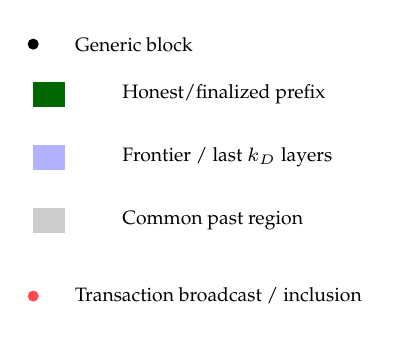
\begin{tikzpicture}[x=1cm,y=0.8cm,>=Latex,thick]

  % Black = blocks
  \fill[black] (0,0) circle (2pt);
  \node[right=0.4cm of {(0,0)}] {\scriptsize Generic block};

  % Green = honest/finalized prefix
  \fill[green!40!black] (0,-1) rectangle (0.4,-0.6);
  \node[right=0.6cm of {(0.4,-0.8)}] {\scriptsize Honest/finalized prefix};

  % Blue = frontier
  \fill[blue!30] (0,-2) rectangle (0.4,-1.6);
  \node[right=0.6cm of {(0.4,-1.8)}] {\scriptsize Frontier / last $k_D$ layers};

  % Gray = common past
  \fill[black!20] (0,-3) rectangle (0.4,-2.6);
  \node[right=0.6cm of {(0.4,-2.8)}] {\scriptsize Common past region};

  % Red = transaction broadcast
  \fill[red!70] (0,-4) circle (2pt);
  \node[right=0.4cm of {(0,-4)}] {\scriptsize Transaction broadcast / inclusion};

\end{tikzpicture}
\caption{\textbf{Legend of colors used in Figures~\ref{fig:dg}--\ref{fig:liveness}.} 
Black = blocks; green = honest or finalized prefix; 
blue = frontier region; gray = common past; red = broadcast transaction event or inclusion.}
\label{fig:legend}
\end{figure}




\subsubsection{DAG Growth (DG)} 
In any window of $\ell$ slots after GST, the number of new honest blocks that become ancestors of at least one honest tip grows linearly: at least $\tau_D \cdot \ell$ new honest blocks are created and confirmed by honest references.




\begin{figure}[htp!]
\centering
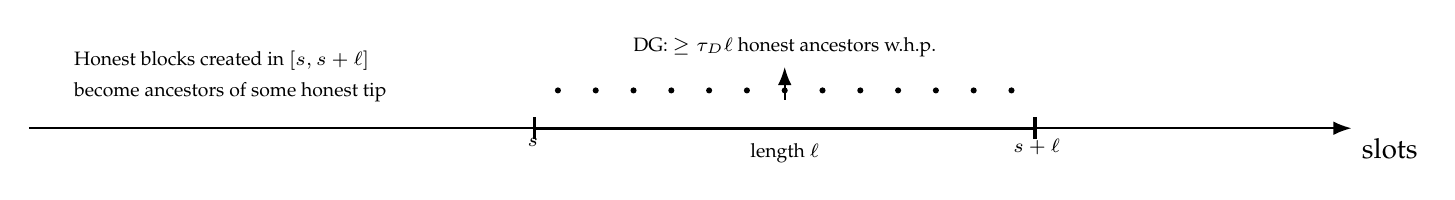
\begin{tikzpicture}[x=0.16cm,y=0.6cm,>=Latex,thick]
  % Axis
  \draw[-{Latex}] (0,0) -- (105,0) node[below right] {slots};

  % Interval [s, s+ell]
  \draw[very thick,|-|] (40,0) -- (80,0);
  \node[below] at (40,0) {\scriptsize $s$};
  \node[below] at (80,0) {\scriptsize $s+\ell$};
  \node[below] at (60,-0.1) {\scriptsize length $\ell$};

  % Honest blocks accumulating
  \foreach \x in {42,45,48,51,54,57,60,63,66,69,72,75,78} {
    \fill[black] (\x,0.8) circle (1.1pt);
  }
  \node[align=left] at (16,1.1) {\scriptsize Honest blocks created in $[s,s+\ell]$ \\[-1pt] \scriptsize become ancestors of some honest tip};

  % Arrow up
  \draw[->] (60,0.6) -- (60,1.3);
  \node[above] at (60,1.3) {\scriptsize DG: $\ge \tau_D\ell$ honest ancestors w.h.p.};
\end{tikzpicture}
\caption{\textbf{DAG Growth (DG).} 
\small
Over any $\ell$-slot interval after GST, at least $\tau_D\ell$ honest blocks become ancestors of some honest tip with probability $1-\negl(\lambda)$. 
Black dots represent honest blocks produced during the interval.}

%\caption{\textbf{DAG Growth (DG).} Over any $\ell$-slot interval after GST, at least $\tau_D\ell$ honest blocks become ancestors of some honest tip with probability $1-\negl(\lambda)$.}
\label{fig:dg}
\end{figure}

\begin{definition}[DAG Growth]
Fix security parameter $\lambda$ and let $\negl(\cdot)$ denote a negligible function.
Let $\mathrm{GST}$ be the global stabilization time and $\Delta$ the post-GST delay bound.
For any interval $I=[s,s+\ell-1]$ of $\ell$ consecutive slots with $s\ge \mathrm{GST}$, let
$H_I$ be the set of honest blocks created in $I$ that, by the end of slot $s+\ell-1+\Delta$, are ancestors of at least one honest tip.
We say $\mathrm{DG}[\tau_D,\ell]$ holds if for all such intervals
\begin{equation*}
\Pr\big[\,|H_I|\ \ge\ \tau_D\cdot \ell\,\big]\ \ge\ 1-\negl(\lambda).
\end{equation*}
\end{definition}


\subsubsection{DAG Quality (DQ)} 
In any window of $\ell$ slots, the fraction of honest blocks among all blocks entering the “recent frontier” (within the last $w$ slots on the preferred branch) is at least $\mu_D$.



\begin{definition}[DAG Quality]
Fix security parameter $\lambda$. For any interval $I=[s,s+\ell-1]$ with $s\ge \mathrm{GST}$, consider the set $B_I$ of blocks that enter the preferred branch's frontier (i.e., become descendants of the fork-choice tip) during $I$. Let $B_I^{\mathsf{H}}$ be those created by honest parties.
We say $\mathrm{DQ}[\mu_D,\ell]$ holds if
\begin{equation*}
\Pr\big[\,|B_I^{\mathsf{H}}|\ \ge\ \mu_D \cdot |B_I|\,\big]\ \ge\ 1-\negl(\lambda).
\end{equation*}
\end{definition}

\begin{figure}[htp!]
\centering
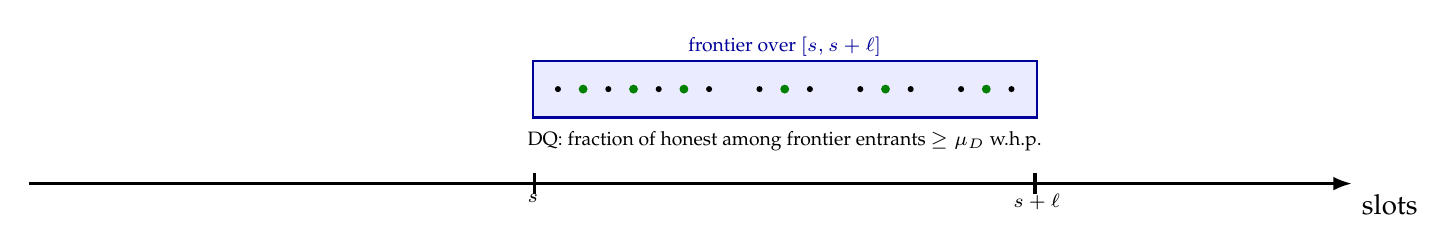
\begin{tikzpicture}[x=0.16cm,y=0.6cm,>=Latex,thick]
  % Axis
  \draw[-{Latex}] (0,0) -- (105,0) node[below right] {slots};

  % Frontier band over an interval
  \fill[blue!8] (40,1.4) rectangle (80,2.6);
  \draw[blue!60!black] (40,1.4) rectangle (80,2.6);
  \node[blue!60!black] at (60,2.9) {\scriptsize frontier over $[s,s+\ell]$};

  % Honest vs total markers in frontier
  \foreach \x in {42,46,50,54,58,62,66,70,74,78} {
    \fill[black] (\x,2.0) circle (1.1pt); % total
  }
  \foreach \x in {44,48,52,60,68,76} {
    \fill[green!50!black] (\x,2.0) circle (1.6pt); % honest subset
  }

  % Labels s and s+ell
  \draw[very thick,|-|] (40,0) -- (80,0);
  \node[below] at (40,0) {\scriptsize $s$};
  \node[below] at (80,0) {\scriptsize $s+\ell$};

  % Callout
  \node[align=center] at (60,0.9) {\scriptsize DQ: fraction of honest among frontier entrants $\ge \mu_D$ w.h.p.};
\end{tikzpicture}
\caption{\textbf{DAG Quality (DQ).} 
\small 
In any $\ell$-slot window after GST, the fraction of \emph{honest blocks} among those entering the advancing frontier is at least $\mu_D$ with probability $1-\negl(\lambda)$. 
In the illustration, the blue band marks the advancing frontier; 
black dots represent all blocks that enter this frontier, 
and green dots highlight the subset created by honest parties.}

%\caption{\textbf{DAG Quality (DQ).} In any $\ell$-slot window after GST, the fraction of honest blocks among those entering the advancing frontier is at least $\mu_D$ with probability $1-\negl(\lambda)$.}
\label{fig:dq}
\end{figure}





\subsubsection{DAG Common Past (DCP)}

For any two honest views of the DAG at times $t_1\le t_2$, if we remove the last $k_D$ layers from the current frontier, the remaining past is identical. Equivalently, all honest parties share the set of ancestors up to the most recent CCA of their tips.




\begin{definition}[DAG Common Past (DCP)]
Fix $k_D \in \mathbb{N}$. For an honest party $P$ at slot $t$, let $V_t^P$ denote
its view of the DAG at the end of $t$, and define
$\mathsf{Trim}(V_t^P,k_D)$ as $V_t^P$ with the last $k_D$ layers (by slots)
beneath its fork-choice tip removed.

We say $\mathrm{DCP}[k_D]$ holds if for all honest parties $P,Q$ and all slots
$t_1 \le t_2$ after $\mathrm{GST}$,
\[
\Pr\!\Big[\, \mathsf{Trim}(V_{t_1}^P,k_D)\;\subseteq\;\mathsf{Trim}(V_{t_2}^Q,k_D)\,\Big]
\;\ge\; 1-\negl(\lambda).
\]
That is, once the most recent $k_D$ layers are trimmed, the earlier view of
any honest party is always contained in the later view of any other honest party,
except with negligible probability.
\end{definition}



\begin{figure}[htbp!]
\centering
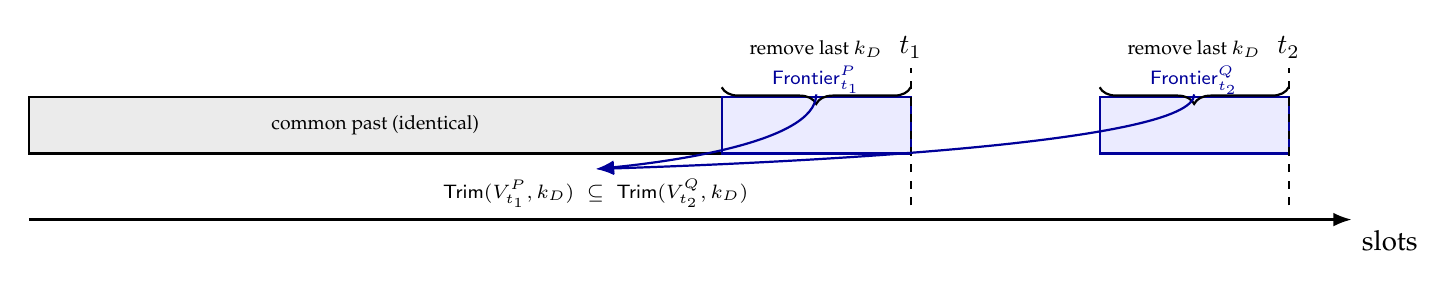
\begin{tikzpicture}[x=0.16cm,y=0.6cm,>=Latex,thick]
  % Axis
  \draw[-{Latex}] (0,0) -- (105,0) node[below right] {slots};

  % Common past region (identical after trimming)
  \fill[black!8] (0,1.4) rectangle (55,2.6);
  \draw (0,1.4) rectangle (55,2.6);
  \node at (27.5,2.0) {\scriptsize common past (identical)};

  % Frontier windows near t1 and t2 (last k_D layers)
  \fill[blue!8] (55,1.4) rectangle (70,2.6);
  \draw[blue!60!black] (55,1.4) rectangle (70,2.6);
  \node[blue!60!black] at (62.5,2.95) {\scriptsize $\mathsf{Frontier}_{t_1}^P$};

  \fill[blue!8] (85,1.4) rectangle (100,2.6);
  \draw[blue!60!black] (85,1.4) rectangle (100,2.6);
  \node[blue!60!black] at (92.5,2.95) {\scriptsize $\mathsf{Frontier}_{t_2}^Q$};

  % Vertical markers t1, t2
  \draw[dashed] (70,0.3) -- (70,3.2) node[above] {$t_1$};
  \draw[dashed] (100,0.3) -- (100,3.2) node[above] {$t_2$};

  % Braces highlighting "trim" operation
  \draw[decorate,decoration={brace,amplitude=6pt}] (70,2.8) -- (55,2.8)
    node[midway,above=7pt] {\scriptsize remove last $k_D$};
  \draw[decorate,decoration={brace,amplitude=6pt}] (100,2.8) -- (85,2.8)
    node[midway,above=7pt] {\scriptsize remove last $k_D$};

  % Annotation showing subset relation of trimmed DAGs
  \node[align=center] (trimEq) at (45,0.55)
    {\scriptsize $\mathsf{Trim}(V_{t_1}^P,k_D)\;\subseteq\;\mathsf{Trim}(V_{t_2}^Q,k_D)$};

  % Arrows from braces to annotation
  \draw[->,blue!60!black] (62.5,2.65) .. controls (62.5,1.6) and (50,1.2) .. (trimEq.north);
  \draw[->,blue!60!black] (92.5,2.65) .. controls (92.5,1.6) and (60,1.2) .. (trimEq.north);

\end{tikzpicture}
\caption{\textbf{DAG Common Past (DCP).} 
The \textcolor{black!60!white}{gray region} shows the common past that all honest parties agree on. 
The \textcolor{blue!60!black}{blue regions} represent the most recent $k_D$ layers 
(\,$\mathsf{Frontier}_{t_1}^P$, $\mathsf{Frontier}_{t_2}^Q$\,) beneath the fork-choice tips at times $t_1\le t_2$. 
By removing these blue frontier layers, the earlier trimmed DAG is always contained in the later one,
i.e., $\mathsf{Trim}(V_{t_1}^P,k_D)\subseteq \mathsf{Trim}(V_{t_2}^Q,k_D)$,
with probability $1-\negl(\lambda)$.}
\label{fig:dcp}
\end{figure}



%\newpage

\subsubsection{Persistence (Safety)}


A protocol has \emph{persistence} with parameter $k$ if for any two honest times $t_1\le t_2$,
the ledgers induced by the fork-choice at those times agree on all transactions that are at least $k$-deep at time $t_1$,
except with probability $\negl(\lambda)$.

\begin{definition}[Persistence (Safety)]
Fix $k \in \mathbb{N}$. For an honest party $P$ and slot $t$, let $L_t^P$ denote
the ledger (totally ordered list of transactions) induced by applying the fork-choice
rule to $V_t^P$. We say $\mathrm{Persistence}[k]$ holds if for all pairs of honest
parties $P,Q$ and all slots $t_1 \le t_2$ after $\mathrm{GST}$,
\[
\Pr\!\Big[\, L_{t_1}^P[1..n-k] \;=\; L_{t_2}^Q[1..n-k] \,\Big] \;\ge\; 1-\negl(\lambda),
\]
where $n=|L_{t_1}^P|$. That is, all but the last $k$ transactions in $P$'s ledger
at time $t_1$ are immutable and appear in $Q$'s ledger at time $t_2$.
\end{definition}

\begin{figure}[htp!]
\centering
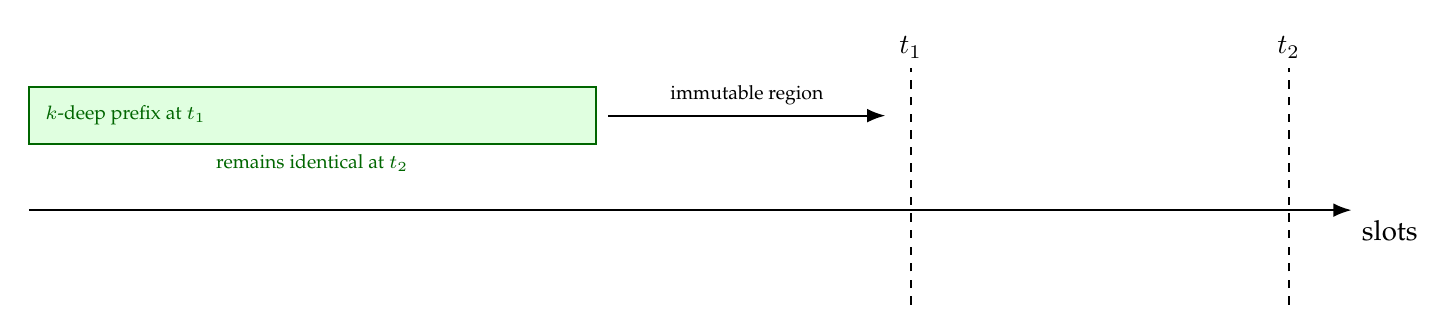
\begin{tikzpicture}[x=0.16cm,y=0.6cm,>=Latex,thick]
  % Axis
  \draw[-{Latex}] (0,0) -- (105,0) node[below right] {slots};

  % t1 and t2 markers
  \draw[dashed] (70,-2.0) -- (70,3.0) node[above] {$t_1$};
  \draw[dashed] (100,-2.0) -- (100,3.0) node[above] {$t_2$};

  % k-deep prefix at t1
  \fill[green!12] (0,1.4) rectangle (45,2.6);
  \draw[green!40!black] (0,1.4) rectangle (45,2.6);
  \node[green!40!black,anchor=west] at (0.5,2.0) {\scriptsize $k$-deep prefix at $t_1$};

  % Same prefix at t2 (visual echo)
  \draw[green!40!black,dashed] (0,1.4) rectangle (45,2.6);
  \node[green!40!black] at (22.5,1.0) {\scriptsize remains identical at $t_2$};

  % Legend arrow
  \draw[->] (46,2.0) -- (68,2.0) node[midway,above] {\scriptsize immutable region};
\end{tikzpicture}
\caption{\textbf{Persistence (Safety).} 
\small 
All but the last $k$ transactions in the ledger at time $t_1$ remain immutable and appear in every honest ledger at any later time $t_2\ge t_1$, except with probability $1-\negl(\lambda)$. 
The green region shows the $k$-deep finalized prefix at $t_1$, which remains unchanged in later ledgers.}

%\caption{\textbf{Persistence (Safety).} All but the last $k$ transactions in the ledger at time $t_1$ appear identically in every honest ledger at any later time $t_2\ge t_1$, except with probability $1-\negl(\lambda)$.}
\label{fig:persistence}
\end{figure}

\subsubsection{Liveness}



A protocol has \emph{liveness} with parameter $\ell_{\mathrm{live}}$ if for any valid transaction broadcast continuously by an honest party,
the transaction appears in the ledger of every honest party within $\ell_{\mathrm{live}}$ slots after $\mathrm{GST}$,
except with probability $\negl(\lambda)$.

\begin{definition}[Liveness]
Fix $\ell_{\mathrm{live}} \in \mathbb{N}$. For any valid transaction $\tx$ that is
broadcast by an honest party $P$ in every slot after $\mathrm{GST}$, let
$E_t^Q(\tx)$ denote the event that honest party $Q$'s ledger $L_t^Q$ at the end of slot $t$
contains $\tx$. We say $\mathrm{Liveness}[\ell_{\mathrm{live}}]$ holds if for all honest parties $P,Q$
and for all slots $s \ge \mathrm{GST}$,
\[
\Pr\!\Big[\, \exists\, t \in [s,\,s+\ell_{\mathrm{live}}] : E_t^Q(\tx) \,\Big] \;\ge\; 1-\negl(\lambda).
\]
In words: any transaction repeatedly injected by an honest party after $\mathrm{GST}$
is guaranteed to appear in every honest party’s ledger within $\ell_{\mathrm{live}}$ slots,
except with negligible probability.
\end{definition}

\begin{figure}[htp!]
\centering
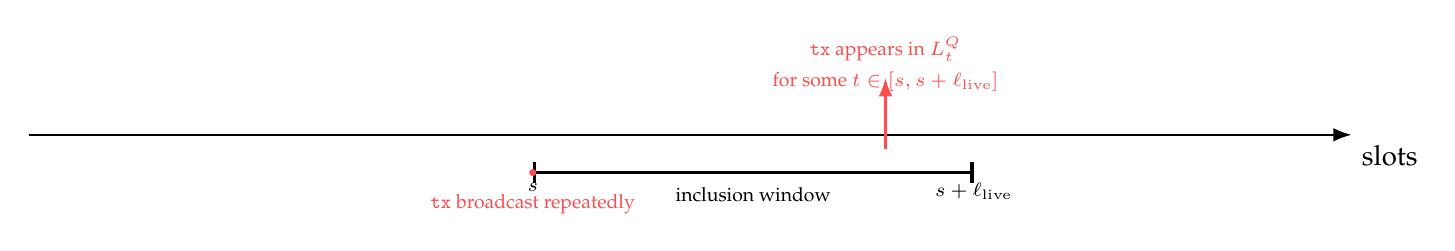
\begin{tikzpicture}[x=0.16cm,y=0.6cm,>=Latex,thick]
  % Axis
  \draw[-{Latex}] (0,0) -- (105,0) node[below right] {slots};

  % Broadcast start s and window [s, s+ell_live]
  \draw[very thick,|-|] (40,-0.8) -- (75,-0.8);
  \node[below] at (40,-0.8) {\scriptsize $s$};
  \node[below] at (75,-0.8) {\scriptsize $s+\ell_{\mathrm{live}}$};
  \node[below] at (57.5,-0.9) {\scriptsize inclusion window};

  % Broadcast event
  \fill[red!70] (40,-0.8) circle (1.3pt);
  \node[below=4pt,red!70] at (40,-0.8) {\scriptsize $\tx$ broadcast repeatedly};

  % Inclusion arrow into ledger
  \draw[->,red!70] (68,-0.3) -- (68,1.2);
  \node[red!70,align=center] at (68,1.5) {\scriptsize $\tx$ appears in $L_t^Q$\\[-1pt]\scriptsize for some $t\in[s,s+\ell_{\mathrm{live}}]$};
\end{tikzpicture}
\caption{\textbf{Liveness.} 
\small
Any valid transaction broadcast continuously by an honest party after GST is included in every honest ledger within $\ell_{\mathrm{live}}$ slots, except with probability $1-\negl(\lambda)$. 
Red marks the transaction broadcast event at slot $s$ and the inclusion window $[s,s+\ell_{\mathrm{live}}]$, with an arrow showing when the transaction enters an honest ledger.}

%\caption{\textbf{Liveness.} Any valid transaction broadcast continuously by an honest party after GST is included in every honest ledger within $\ell_{\mathrm{live}}$ slots, except with probability $1-\negl(\lambda)$.}
\label{fig:liveness}
\end{figure}





\subsection{Tip Boundedness and Its Necessity}
\label{subsec:tip-boundedness}

The preceding invariants (DAG Growth, DAG Quality, DAG Common Past) capture progress, fairness, and eventual agreement on history. However, these three alone are insufficient to guarantee a secure ledger. We introduce the additional invariant of \emph{Tip Boundedness} (TB).

\begin{definition}[Tip Boundedness]
A protocol satisfies $\mathrm{TB}[\beta]$ if, at any time after GST, the number of incomparable honest tips is at most $\beta$, except with negligible probability. 
Here $\beta$ is $O(\Delta \cdot \text{block rate})$, i.e., proportional to the maximum number of honest blocks that can be created during the delay window $\Delta$.
\end{definition}

\paragraph{Why TB Is Necessary.}
If the number of honest tips is unbounded, then:
\begin{itemize}
  \item \textbf{Safety problem:} honest work fragments across many incomparable branches. In fork-choice, this allows an adversary to amplify one branch with concentrated weight, overriding other honest branches. Even if DAG Growth, DAG Quality, and DAG Common Past hold, safety fails because no branch accumulates stable majority weight.
  \item \textbf{Liveness problem:} some honest blocks may remain stranded: if new tips appear faster than they can be merged, many honest transactions never receive enough descendants to be included in the common past. Liveness then fails, even though the DAG continues to grow.
\end{itemize}

\begin{lemma}[Necessity of TB for Ledger Properties]
DAG Growth, DAG Quality, and DAG Common Past are insufficient to imply persistence and liveness of the ledger. In particular, without Tip Boundedness, there exist adversarial schedules where (i) some honest blocks never accumulate any confirming descendants (breaking liveness), and (ii) two branches each accumulate enough honest blocks to satisfy DG, DQ, DCP, yet neither dominates, allowing divergent ledgers (breaking safety).
\end{lemma}

\begin{proof}[Proof sketch]
In a DAG where honest proposers perpetually extend different tips (e.g., due to unpredictable network delays), both branches keep growing linearly (DG holds) and each sees an honest fraction (DQ holds), and occasional cross-references ensure a large common prefix (DCP holds). However, if tips are never fully merged (no TB), then each branch might have infinitely many honest blocks without one outweighing the other. One can construct a schedule where two honest groups alternate making tips, resulting in a DAG with two ``stalemated'' superchains. Honest transactions included in one branch never appear in the ledger of parties following the other branch (violating liveness), and a block confirmed in one branch can be overturned by the other branch’s growth (violating persistence).
\end{proof}


\paragraph{Remark: TB vs.\ DCP and Relation to Long-Delay Attacks.}
It is important to note that DAG Common Past (DCP) does \emph{not} imply Tip
Boundedness (TB). DCP ensures that if one trims away the most recent $k_D$ layers,
then all honest views coincide on the older prefix. However, DCP does not constrain
how many incomparable tips may exist within those last $k_D$ layers. In particular,
one can have a DAG where the deep past is fully common (DCP holds), yet the active
frontier contains $\Theta(\Delta \cdot \text{block rate})$ or even unboundedly many
tips. Thus, persistence and liveness may fail even though DG, DQ, and DCP all hold:
the honest work is fragmented across too many branches to form a stable margin.

This observation parallels the \emph{long-delay attack} described by Pass, Seeman,
and shelat in their analysis of Nakamoto consensus in asynchronous networks~\cite[Section 8]{EC:PasSeeShe17}. They show that when
network delays are large relative to block production, the honest chain fragments
into many concurrent forks, which an adversary can exploit to cause deep reorgs.
Our TB property directly precludes such fragmentation in DAG protocols: it enforces
a bound on the width of the tip set, thereby ensuring that honest references
continually collapse the frontier. In this sense, TB can be viewed as the DAG
analogue of the synchrony assumption needed to rule out long-delay attacks in
chain-based protocols.

%%%%%%%%%%%%%%%%%%%%%%%%%%%%%%%%%%%%%%%%%%%%%%%%%%%%%%%%%%%%%%%%%%%%%%%%%%%%%%%
% Section 3: Cryptareon-Ideal (NEW)
%%%%%%%%%%%%%%%%%%%%%%%%%%%%%%%%%%%%%%%%%%%%%%%%%%%%%%%%%%%%%%%%%%%%%%%%%%%%%%%
\section{Cryptareon-Ideal: Idealized Multi-Proposer Protocol (NEW)}
\label{sec:ideal}

\subsection{Overview and Assumptions}
\label{subsec:ideal-overview}
\ProjIdeal isolates the core consensus logic of a leaderless, multi-proposer DAG protocol to enable crisp arguments about safety and liveness. The model makes the following simplifying assumptions:
\begin{itemize}
  \item \textbf{Synchronous delivery:} time proceeds in slots; all honest messages broadcast in slot $s$ are delivered to all honest parties by the end of slot $s$ (zero-latency abstraction).
  \item \textbf{Public-coin eligibility:} each validator $v\in\Val$ independently becomes eligible in slot $s$ with probability $p\cdot\stakefrac{v}$ (a public-coin surrogate for VRF sortition).
  \item \textbf{Unbounded referencing:} when eligible, an honest block may reference \emph{any} existing block(s). Honest creators attempt to cite \emph{all} currently visible tips (equivalently, a maximum antichain).\footnote{Exact vs.\ greedy antichain selection is discussed; both are admissible in \ProjIdeal.}
  \item \textbf{Bounded fork-choice window:} \emph{weight} used in fork choice counts only references created within a fixed \emph{window} of most recent slots (window length $w\ge1$). This prevents long-range withholding from dominating fork choice (\S\ref{subsec:ideal-window-justification}).
  \item \textbf{No transaction conflicts / slashing:} to focus on consensus dynamics, we idealize away UTXO conflicts and slashing; each validator produces at most one block per slot by definition.
\end{itemize}

\vspace{0.25em}
\noindent\textbf{Notation.}
We reuse the global notation from Section~\ref{sec:model}. The reference DAG is $G=(V,E)$ with $u\leadsto v$ denoting reachability. $\Tips(G)$ is the set of vertices of out-degree $0$.

\subsection{Algorithms (for reference)}
We recall the algorithms already presented:
\begin{itemize}
  \item \textbf{Alg.~\ref{alg:ideal-antichain}} (\emph{AntichainSelection}): compute a (maximum or greedy) antichain of the current DAG.
  \item \textbf{Alg.~\ref{alg:ideal-create}} (\emph{Block Creation}): if eligible in slot $s$, build a block that references the selected antichain and broadcast it.
  \item \textbf{Alg.~\ref{alg:ideal-reception}} (\emph{Block Reception}): integrate a valid incoming block; update $\Tips$ and fork-choice state.
  \item \textbf{Alg.~\ref{alg:ideal-anchored-fc}} (\emph{Anchored Fork Choice}): score candidate tips by window-filtered reference weight anchored at $a$; pick the maximum.
  \item \textbf{Alg.~\ref{alg:ideal-cca}} (\emph{Conflict Resolution via CCA}): for conflicting heads $i,j$, anchor at $c=\CCA(i,j)$ and compare window-filtered branch weights; choose the heavier branch.
\end{itemize}

\subsection{Protocol Walkthrough (Honest Player View)}
\label{subsec:ideal-walkthrough}
This subsection explains how an \emph{honest} validator executes \ProjIdeal in each slot, and how fork choice and conflict resolution interplay with block creation and reception.

\paragraph{Per-slot loop (local state machine).}
At the beginning of slot $s$, an honest player $P$ has local DAG $G_s=(V_s,E_s)$:
\begin{enumerate}
  \item \textbf{Eligibility check.} $P$ samples public coins for slot $s$ and determines eligibility with probability $p\cdot\stakefrac{P}$.
  \item \textbf{Reference selection (Alg.~\ref{alg:ideal-antichain}).} $P$ deterministically computes an antichain $A_s\subseteq V_s$. In \ProjIdeal, $A_s$ may include \emph{all} current tips since referencing is unbounded.
  \item \textbf{Block creation (Alg.~\ref{alg:ideal-create}).} If eligible, $P$ constructs block $b_s=\langle \id,\val{=}P,\slot{=}s,\txs,\refs{=}A_s\rangle$ and broadcasts $b_s$.
  \item \textbf{Block reception and integration (Alg.~\ref{alg:ideal-reception}).} Throughout the slot and by its end, $P$ receives all blocks broadcast in slot $s$. For each block $b$ not yet in $V_s$, $P$ verifies well-formedness and acyclicity, inserts $b$ and edges $(r\to b)$ for all $r\in\refs(b)$, updates $\Tips(G)$ and incremental reachability summaries, and triggers \ForkChoiceUpdate.
  \item \textbf{Fork choice (Alg.~\ref{alg:ideal-anchored-fc}).} After integrating all blocks for slot $s$, $P$ runs anchored fork choice: for anchor $a$ (genesis or last finalized checkpoint), it computes window-filtered scores $W(T)$ for each $T\in\Tips(G)$ and sets the preferred tip $\hat{T}_s$ to the maximizer. The \emph{ledger view} of $P$ at the end of slot $s$ is the linearization induced by the preferred branch to $\hat{T}_s$.
  \item \textbf{Conflict resolution (Alg.~\ref{alg:ideal-cca}).} If two incomparable blocks $i,j$ imply conflicting ledger states above some ancestor, $P$ computes $c=\CCA(i,j)$ and compares window-filtered branch weights $\BranchW(i;c,w)$ vs.\ $\BranchW(j;c,w)$ to decide the winner. This rule is \emph{consistent} with the anchored fork choice: the preferred tip must lie on the heavier branch as measured from their CCA.
\end{enumerate}



\paragraph{Finalization rule (informal).}
In \ProjIdeal, blocks become \emph{finalized} purely through the fork-choice dynamics,
without requiring any separate BFT-style gadget.
Specifically, an honest party may treat a block as final once it is
$k$-deep under the current preferred tip, for a parameter
$k=k(w,\epsilon)$ established in the safety analysis
(\S\ref{subsec:ideal-ledger-props}).
Intuitively, once a block has accumulated sufficient window-filtered weight,
any conflicting branch beyond the relevant CCA cannot overtake it,
since adversarial work created outside the last $w$ slots has no effect.

\begin{remark}[Comparison with BFT-style finality]
Traditional BFT-based protocols (e.g., HotStuff, Casper FFG) achieve finality
through explicit voting and quorum certificates.
In contrast, our design provides \emph{probabilistic finality} directly from
the weight-based fork-choice and bounded-window analysis:
a block becomes irreversible once its depth ensures an honest margin
that no adversary with $\alpha < 1/2$ stake can overcome.
Thus, finality emerges organically from the ledger’s growth properties,
without any auxiliary consensus layer.
\end{remark}

\subsection{On Unbounded Referencing vs.\ Bounded Fork Choice}
\label{subsec:ideal-window-justification}
\ProjIdeal allows \emph{unbounded referencing}: an honest block may cite \emph{all} existing tips (or a maximum antichain), which accelerates convergence and directly implies Tip Boundedness (TB) in the synchronous ideal.
However, using \emph{unbounded} weight in fork choice (i.e., counting all references since genesis) is unsafe even in a synchronous model because an adversary can \emph{withhold} a private subtree for many slots and then reveal it at once. The revealed descendants would contribute large cumulative score to an adversarial branch, potentially overriding the honest branch despite minority stake.

\begin{lemma}[Unsafe infinite-horizon weight]
Even under synchrony and honest majority, if fork choice scores branches by \emph{unbounded} descendant counts since genesis, there exists a withholding strategy that can cause arbitrarily deep reversions with non-negligible probability.
\end{lemma}

\begin{proof}[Proof sketch]
Let the adversary with stake fraction $\alpha<1/2$ privately build a subtree extending from a recent CCA while the honest parties continue extending the public branch. After $L$ slots, the private subtree accumulates $\Theta(\alpha L)$ references while the honest branch accumulates $\Theta((1-\alpha)L)$. If the scoring aggregates from genesis, the adversary can time its release to coincide with honest fragmentation at the frontier (many tips), so the adversarial branch appears heavier due to concentrated weight. Since contributions are not window-limited, the \emph{entire} private accumulation applies, enabling deep reorgs. Window-filtering neutralizes this leverage by discarding stale contributions outside the last $w$ slots.
\end{proof}

\noindent\textbf{Conclusion.} In \ProjIdeal we \emph{retain unbounded referencing} (for rapid merging and TB), but we \emph{require a bounded window $w$ in the fork-choice metric}. This pairing preserves fast convergence while preventing long-range weight accumulation from withheld blocks.

\subsection{Security of the Idealized Protocol}
\label{subsec:ideal-security}
We now prove that \ProjIdeal satisfies the DAG invariants (DG, DQ, DCP, TB) and, consequently, \emph{ledger persistence (safety)} and \emph{liveness}. Throughout, let the honest stake fraction be $H\in(1/2,1]$ and let $p\in(0,1]$ be the per-slot eligibility rate (public-coin). All statements hold \emph{except with negligible probability} in the security parameter $\lambda$ (via Chernoff-type bounds).

\paragraph{Preliminaries.} In slot $s$, the number of honest eligible validators is $\mathrm{Hon}_s\sim \mathrm{Binomial}(|\Val|,\,p\cdot \mathbb{E}[\stakefrac{v}\,|\,v\text{ honest}])$, with expectation $\Theta(pH|\Val|)$. Under synchrony and unbounded referencing, all blocks created in slot $s$ can reference \emph{all tips visible at the start of the slot}, and all honest parties receive the same set of blocks by the end of the slot.

\begin{theorem}[DAG Growth (DG) in \ProjIdeal]
\label{thm:ideal-DG}
Fix any interval of $\ell$ slots after GST. With probability $1-\negl(\lambda)$, at least $\tau_D\ell$ honest blocks are created and become ancestors of some honest tip by the end of the interval, for $\tau_D=\Theta(pH)$.
\end{theorem}
\begin{proof}[Proof sketch]
Linearity and Chernoff concentration on $\sum_{s} \mathrm{Hon}_s$ give $\Theta(pH\ell)$ honest blocks in the interval. Under synchrony, each of these blocks is referenced by subsequent honest blocks in the next slot, hence becomes an ancestor of an honest tip. 
\end{proof}

\begin{theorem}[DAG Quality (DQ) in \ProjIdeal]
\label{thm:ideal-DQ}
For any $\ell$-slot window after GST, the fraction of honest blocks entering the preferred frontier is at least $\mu_D=\Theta(H)$ with probability $1-\negl(\lambda)$.
\end{theorem}
\begin{proof}[Proof sketch]
Eligibility is stake-proportional and independent across validators; thus the expected honest fraction per slot is $H$. Since fork-choice is deterministic and anchored, the selection process does not bias adversarial blocks upwards; Chernoff bounds imply concentration around $H$ over $\ell$ slots.
\end{proof}

\begin{theorem}[Tip Boundedness (TB) in \ProjIdeal]
\label{thm:ideal-TB}
With unbounded referencing and synchrony, $\mathrm{TB}[\beta]$ holds with $\beta=O(p\,|\Val|)$.
\end{theorem}
\begin{proof}[Proof sketch]
At most $O(p\,|\Val|)$ honest blocks are created in a slot; each of them references \emph{all} pre-existing tips, so all prior tips are buried and removed from $\Tips(G)$. Thus the tip set after each slot is bounded by the number of new blocks created in that slot.
\end{proof}

\begin{theorem}[DAG Common Past (DCP) in \ProjIdeal]
\label{thm:ideal-DCP}
There exists $k_D=O(1)$ such that removing the last $k_D$ layers beneath each honest party's preferred tip yields identical ancestor sets, with probability $1-\negl(\lambda)$.
\end{theorem}
\begin{proof}[Proof sketch]
Synchrony implies identical views at the end of each slot. By TB, the frontier width is $O(1)$ (in expectation and with exponential tails). Because honest blocks in slot $s{+}1$ reference all tips from slot $s$, any divergence confined to the last $O(1)$ layers is reconciled in one step. Hence $k_D=O(1)$ suffices.
\end{proof}

\subsubsection*{Ledger Properties (Persistence and Liveness)}
\label{subsec:ideal-ledger-props}
We now show that \ProjIdeal's anchored, window-filtered fork choice, coupled with CCA-based conflict resolution, yields ledger safety and liveness.

\begin{theorem}[Persistence (Safety) of \ProjIdeal]
\label{thm:ideal-safety}
There exists $k=k(w,\epsilon)$ such that if a block $B$ is $k$-deep under the preferred tip of an honest party at the end of some slot, then with probability $1-\negl(\lambda)$, $B$ remains in the ledger of all honest parties at all future times (no conflicting ledger can supersede it).
\end{theorem}
\begin{proof}[Proof sketch]
Consider any conflicting branch revealed later whose head $j$ competes against the honest head $i$ after their CCA $c=\CCA(i,j)$. By DG, DQ, and TB, the honest branch accumulates $\Omega(w)$ window-filtered references in the next $w$ slots. Since fork choice counts only the last $w$ slots anchored at $c$, any adversarial references created \emph{more than $w$ slots} ago (e.g., withheld) contribute zero score. Thus, once the honest branch leads by a margin growing with $w$, the adversary cannot overturn it without controlling $\ge 1/2$ of stake \emph{within the window}. Choosing $k=\Theta(w)$ ensures this margin has formed \emph{before} $B$ is declared final, yielding persistence.
\end{proof}

\begin{theorem}[Liveness of \ProjIdeal]
\label{thm:ideal-liveness}
For any valid transaction $\tx$ broadcast by an honest party after GST, there exists $\ell_{\mathrm{live}}=\mathrm{poly}(1/p,1/H)$ such that $\tx$ appears in the ledger of every honest party within $\ell_{\mathrm{live}}$ slots, except with negligible probability.
\end{theorem}
\begin{proof}[Proof sketch]
In each slot, with constant probability at least one honest validator is eligible; upon eligibility, the validator can include $\tx$. Under synchrony and unbounded referencing, subsequent honest blocks reference the block containing $\tx$ and quickly bury it. Using DG, DQ, and TB, the block's descendant count grows linearly over time, and the window-filtered fork choice maintains the branch as preferred, so $\tx$ enters all honest ledgers within $O(\log(1/\negl))$ slots; optimizing constants yields $\ell_{\mathrm{live}}=\tilde{O}(1/(pH))$.
\end{proof}

%%%%%%%%%%%%%%%%%%%%%%%%%%%%%%%%%%%%%%%%%%%%%%%%%%%%%%%%%%%%%%%%%%%%%%%%%%%%%%%
% Section 4: Cryptareon-Base (NEW)
%%%%%%%%%%%%%%%%%%%%%%%%%%%%%%%%%%%%%%%%%%%%%%%%%%%%%%%%%%%%%%%%%%%%%%%%%%%%%%%
\section{Cryptareon-Base: A Practical DAG-Based PoS Protocol (NEW)}
\label{sec:cryptareon-base}

\subsection{Overview and Assumptions (Instantiation of \ProjIdeal)}
\label{subsec:base-overview}
\ProjBase is a practical instantiation of \ProjIdeal (Section~\ref{sec:ideal}) under \emph{partial synchrony} with \emph{VRF sortition}, \emph{bounded short references} (window $w$), and an \emph{optional} single long reference for connectivity. Transactions obey UTXO validity; equivocation is slashable. We retain the \emph{anchored, window-filtered} fork-choice and the \emph{CCA-local} conflict rule.

\begin{itemize}
  \item \textbf{Network.} There exists GST after which honest messages are delivered within $\Delta$ slots.
  \item \textbf{Eligibility.} Each validator $v$ is eligible in slot $s$ iff $(y,\pi)=\VRFSign_{\sk_v}(\domsep\|\chainid\|\netid\|s)$ satisfies $y<p(s,v)$ (Alg.~\ref{alg:block-creation}).
  \item \textbf{References.} In slot $s$, short references must lie in the \emph{window} $W(s;w)=[s{-}w{+}1,s]$; at most one \emph{long-ref} $\ell$ to any older block is allowed and carries zero weight.
  \item \textbf{Fork-choice.} We score tips by summing (optionally stake-weighted) short-reference counts of \emph{descendants} within the last $w$ slots, anchored at a fixed block $a$ (Alg.~\ref{alg:fork-choice}).
  \item \textbf{Conflicts.} Two incomparable blocks implying conflicting ledger states are resolved by comparing window-filtered branch weights \emph{from their} $c=\CCA(i,j)$ (Alg.~\ref{alg:cca-resolve}).
\end{itemize}

\paragraph{Parameter discipline.} Throughout the analysis we assume
\begin{equation}
\label{eq:base-params}
w \;\ge\; \Delta \;+\; \omega(\log\lambda) \qquad\text{and}\qquad 
H>\tfrac{1}{2}+\varepsilon
\end{equation}
for some constant $\varepsilon>0$. The slack $\omega(\log\lambda)$ is used for concentration bounds.

\subsection{Protocol Explanation (Honest Player View: when Algs.~6–9 run)}
\label{subsec:base-walkthrough}
We describe the per-slot state machine of an \emph{honest} node $P$; we explicitly indicate where Algorithms~\ref{alg:block-creation}–\ref{alg:cca-resolve} are invoked. (Depending on global numbering these appear as Algorithms~6–9.)

\paragraph{Start of slot $s$.}
$P$ maintains a local DAG $G_s=(V_s,E_s)$ and a ledger state view induced by its \emph{preferred tip}. It also caches reachability summaries and a per-validator latest-block map.

\begin{enumerate}
  \item \textbf{Eligibility \& transaction sampling.}
  $P$ computes $(\mathsf{ok},\pi,y)\leftarrow\Eligibility(P,s)$. If $\mathsf{ok}=\textsf{true}$, $P$ samples a candidate transaction set $T$ from the mempool (deterministic PRF subsampling seeded by $y$) and prunes conflicts w.r.t.\ current ancestors (UTXO validity).

  \item \textbf{Reference selection (short \& long).}
  $P$ computes a \emph{deterministic} large antichain $R\subseteq V_{s,w}$ of recent blocks (e.g., \GreedyAntichain). If needed for connectivity, it chooses an \emph{optional} long-ref $\ell$ (e.g., last finalized checkpoint). By rule, $|R_{\text{out}}|\le1$ and the long-ref \emph{never} contributes weight.

  \item \textbf{Block creation and gossip (Alg.~\ref{alg:block-creation}).}
  If eligible and after validity checks, $P$ assembles
  \[
  b=\langle 
\id,\val{=}P,\slot{=}s,\txs{=}T,\refs{=}R\cup\{\ell\},y,\pi,\sigma\rangle,
  \]
  signs it, inserts it locally, and gossips.

  \item \textbf{Block reception (Alg.~\ref{alg:block-reception}, continuous during slot).}
  For each received block $b'$: verify VRF proof and signature; fetch missing parents; check (i) window constraint for short refs, (ii) at most one long-ref, (iii) no cycles, (iv) $R_w$ is an antichain in $G_{s,w}$, and (v) no UTXO conflicts vs.\ ancestors. Reject if any check fails; otherwise integrate and update summaries and $\Tips(G)$.

  \item \textbf{Anchored fork-choice (Alg.~\ref{alg:fork-choice}, end of slot).}
  With anchor $a$ (genesis or last finalized checkpoint), compute for each tip $T\in\Tips(G)$ the window-filtered score
  \[
  W(T)=\sum_{\substack{d\in\Desc^*(T)\\a\leadsto d}}\mathrm{contrib}(d)\cdot \wref(d;w),
  \]
  set preferred tip $\hat T_s\in\arg\max W(T)$ (tie-break by $(\slot,\id)$), and expose the induced ledger order.

  \item \textbf{Conflict resolution via CCA (Alg.~\ref{alg:cca-resolve}, on demand).}
  When two incomparable heads $i,j$ imply conflicting states, $P$ computes $c=\CCA(i,j)$ and compares $\BranchW(i;c,w)$ vs.\ $\BranchW(j;c,w)$. The winner determines which subtree remains eligible for inclusion in the preferred branch. This decision is \emph{consistent} with the anchored fork-choice (the preferred tip must lie on the heavier branch past the CCA).
\end{enumerate}

\paragraph{Finalization heuristic.}
$P$ may \emph{finalize} a block $B$ once it is $k$-deep under $\hat T_s$, with $k=\Theta(w)$ as derived in Theorem~\ref{thm:base-safety}. (Finalization is monotone and checkpoint-compatible.)

\subsection{Security of the Practical Protocol}
\label{subsec:base-security}
We prove the DAG invariants and ledger properties for \ProjBase under~\eqref{eq:base-params}. We write $\lambda_h \triangleq \mathbb{E}[\#\text{honest eligible per slot}]=\Theta(pH|\Val|)$.

\subsubsection*{Consensus properties: DG, DQ, TB, DCP}
\begin{theorem}[DAG Growth (DG) in \ProjBase]
\label{thm:base-DG}
For any interval of $\ell$ slots after GST, at least $\tau_D\ell$ honest blocks become ancestors of some honest tip by time $s{+}\ell{-}1{+}\Delta$, with probability $1-\negl(\lambda)$, for $\tau_D=\Theta(pH)$.
\end{theorem}
\begin{proof}[Proof sketch]
Post-GST, in each slot $s$ the number of honest eligible is $\mathrm{Bin}(|\Val|,p\cdot \stakefrac{\cdot})$; Chernoff concentration gives $\Omega(\lambda_h)$ honest blocks per slot over $\ell$ slots. Delivery within $\Delta$ ensures these blocks are referenced by subsequent honest blocks inside the window $w\ge \Delta$, hence they become ancestors of honest tips.
\end{proof}

\begin{theorem}[DAG Quality (DQ) in \ProjBase]
\label{thm:base-DQ}
Fix any $\ell\ge \Omega(\log\lambda)$ after GST. The fraction of honest blocks among those entering the preferred frontier during the interval is at least $\mu_D=\Theta(H)$ w.h.p.
\end{theorem}
\begin{proof}[Proof sketch]
VRF eligibility is stake-proportional; the expected honest fraction per slot is $H$. Window-filtered anchored scoring does not amplify adversarial inputs beyond the window; by linearity and concentration over $\ell$ slots the realized fraction stays within a small deviation of $H$.
\end{proof}

\begin{theorem}[Tip Boundedness (TB) in \ProjBase]
\label{thm:base-TB}
Assume $w\ge \Delta$. Then $\mathrm{TB}[\beta]$ holds with $\beta=O(\lambda_h\cdot \Delta)$ w.h.p.
\end{theorem}
\begin{proof}[Proof sketch]
Within any $\Delta$-slot horizon, honest blocks produced without mutual visibility may introduce multiple tips. After at most $\Delta$ slots these blocks are delivered and subsequent honest blocks (in slots $>s{+}\Delta$) reference \emph{all} visible recent tips within the window, merging them. Hence the tip set size is stochastically dominated by the number of honest blocks created within the last $\Delta$ slots, i.e., $O(\lambda_h\Delta)$, up to lower-order adversarial contributions that are also merged once visible.
\end{proof}

\begin{theorem}[DAG Common Past (DCP) in \ProjBase]
\label{thm:base-DCP}
There exists $k_D=\Theta(\Delta)$ such that, after removing the last $k_D$ layers under the preferred tips of any two honest parties, the remaining ancestor sets coincide w.h.p.
\end{theorem}
\begin{proof}[Proof sketch]
By TB, the honest frontier has bounded width $O(\lambda_h\Delta)$. After $\Delta$ slots, all honest blocks from earlier slots are visible to all honest parties and get cross-referenced within the window, causing the CCA between any two preferred tips to move forward monotonically. Trimming the last $\Theta(\Delta)$ layers removes the area where asynchrony can cause transient divergence, leaving an identical common past.
\end{proof}

\subsubsection*{Ledger properties: Persistence and Liveness}
\begin{theorem}[Persistence (Safety) of \ProjBase]
\label{thm:base-safety}
Let $k=\Theta(w)$ be chosen so that in $w$ slots the honest branch accumulates a fixed constant margin of window-filtered weight against any competing branch past the same CCA. If a block $B$ is $k$-deep under an honest party's preferred tip at time $t$, then with probability $1-\negl(\lambda)$, $B$ remains in every honest party's ledger at all later times.
\end{theorem}
\begin{proof}[Proof sketch]
Consider a conflicting head $j$ and honest head $i$ with $c=\CCA(i,j)$. By DG, DQ, and TB, during any $w$-slot window after $c$ the honest branch contributes $\Omega(\lambda_h w)$ window-filtered references; the adversary contributes $O(\alpha |\Val| p w)$ \emph{only} to blocks \emph{actually created} within the window (withheld older references carry zero weight). Since $H>\tfrac{1}{2}{+}\varepsilon$, the honest margin in the window is positive with high probability and grows with $w$. After $k=\Theta(w)$ depth, any tie can no longer be reached by adversarial scheduling; anchored fork-choice and CCA resolution keep selecting the honest branch, preserving $B$.
\end{proof}

\begin{theorem}[Liveness of \ProjBase]
\label{thm:base-liveness}
For any valid transaction $\tx$ broadcast after GST, there exists $\ell_{\mathrm{live}}=\tilde{O}\!\left( \frac{1}{pH} + \Delta \right)$ such that $\tx$ is included in the ledger of all honest parties within $\ell_{\mathrm{live}}$ slots, except with negligible probability.
\end{theorem}
\begin{proof}[Proof sketch]
With probability $\Omega(pH)$ per slot, some honest validator is eligible and can include $\tx$. Within $\Delta$ slots, the block diffuses to all honest parties; within additional $O(w)$ slots (with $w\ge \Delta$) subsequent honest blocks reference and bury it. The anchored, window-filtered fork-choice maintains the branch as preferred (Theorem~\ref{thm:base-safety}), so $\tx$ propagates to all honest ledgers within $\tilde{O}(1/(pH)+\Delta)$.
\end{proof}

\subsection{Coupling to the Idealized Analysis}
\label{subsec:base-coupling}
\ProjBase is a refinement of \ProjIdeal: unbounded referencing is replaced with \emph{window-bounded} short references plus an \emph{optional} long-ref; public coins are realized with VRFs; synchrony is relaxed to partial synchrony with $w\ge \Delta$. The proofs above adapt the arguments of Section~\ref{sec:ideal} by (i) adding $\Delta$-slot delivery delays in the TB and DCP lemmas; (ii) ensuring that window-filtered weights ignore stale withheld work; and (iii) using stake-proportional VRF concentration for DQ. Thus, each ideal lemma has a practical analogue with slightly weaker (but still constant) parameters.

\subsection{Design Soundness: Remarks and Additional Concerns}
\label{subsec:base-remarks}
\begin{remark}[Window size vs.\ delay]
If $w<\Delta$, honest tips can \emph{expire} from the short-reference window before cross-linking, violating TB and undermining DCP and safety. Hence the constraint $w\ge \Delta$ is \emph{necessary}.
\end{remark}

\begin{remark}[Optional long-ref policy]
Long-refs guarantee global connectivity but carry zero weight. Implementations should \emph{deterministically} choose $\ell$ (e.g., last finalized checkpoint or the $\prec$-max ancestor of the smallest short-ref) to avoid adversarial steering and to enable fast parent fetching.
\end{remark}

\begin{remark}[Slashing condition]
If a validator is caught producing two blocks in the same slot (equivocation), a slashable event occurs. In \ProjBase, such misbehavior can be detected by comparing signatures or VRF proofs. An honest observer can include a special transaction containing $(\id(b),\id(b'),y(b),y(b'),\pi(b),\pi(b'),\sigma(b),\sigma(b'))$ in the ledger to slash $v$'s stake. This disincentivizes equivocation (except short-range attempts, which still yield no gain as they do not increase branch weight beyond the current window).
\end{remark}

\subsection{Discussion of Security and Parameters}
\noindent
\textbf{Safety:} The combination of antichain reference rules, UTXO conflict checks, and the CCA-anchored fork choice ensures that once honest blocks gain a majority of in-window weight over any adversarial branch, the honest branch will prevail. The defined invariants (DG/DQ/DCP/TB) hold with high probability under the usual honest majority assumptions and appropriate parameter choices, leading to persistence.

\smallskip

\noindent
\textbf{Liveness:} By allowing multiple proposers, the protocol increases the rate at which honest votes (references) are cast, helping convergence even with latency. The sliding window (with $w$ sufficiently large relative to $\Delta$) absorbs network delays. Occasional long-refs ensure the DAG does not fragment. Thus, any valid transaction will eventually be included and confirmed.

\smallskip

\noindent
\textbf{Resistance to Withholding:} Because we only count in-window references anchored at the CCA, an adversary cannot secretly build a long private branch that overtakes the honest public branch upon revelation. Withholding yields no advantage once honest blocks keep referencing the honest tips.

\smallskip

\noindent
\textbf{Parameter Choices:} A window on the order of tens of slots (e.g., $w\approx 30$) typically suffices to cover network latency for a moderate honest block rate. The parallelism factor $N_{\MCP}$ tunes how many transactions each block samples, balancing leaderless throughput with verifier load.

\subsection{Cross-Section Correspondence (Sections 3 vs 4)}
The following summary illustrates how the idealized protocol maps to \ProjBase:
\begin{itemize}
  \item \textbf{Eligibility:} Ideal uses implicit Bernoulli coins per slot; Base uses VRF-based eligibility (see Algorithms~\ref{alg:ideal-create}, \ref{alg:block-creation}).
  \item \textbf{Antichain selection:} Ideal selects an exact max antichain (Alg.~\ref{alg:ideal-antichain}); Base uses a greedy antichain within the window (or exact if feasible).
  \item \textbf{Long reference:} Ideal has none ($\OptionalLongRef$ always returns $\bot$); Base allows one deterministic long-ref outside the window.
  \item \textbf{Block creation:} Ideal ignores dependencies and VRFs (Alg.~\ref{alg:ideal-create}); Base includes VRF proof, UTXO conflict checks, and optional long-ref (Alg.~\ref{alg:block-creation}).
  \item \textbf{Block reception:} Ideal only checks acyclicity and parent presence (Alg.~\ref{alg:ideal-reception}); Base verifies VRF/signature, window/antichain constraints, and UTXO validity (Alg.~\ref{alg:block-reception}).
  \item \textbf{Fork choice:} Ideal uses anchored fork choice with unit weights (Alg.~\ref{alg:ideal-anchored-fc}); Base optionally stake-weights references and anchors to finalized checkpoints (Alg.~\ref{alg:fork-choice}).
  \item \textbf{Conflict resolution:} Ideal and Base use the same CCA-based rule (Alg.~\ref{alg:ideal-cca} vs \ref{alg:cca-resolve}), with Base optionally stake-weighting.
\end{itemize}




%%%%%%%%%%%%%%%%%%%%


\section{Implementation and Evaluation}
\label{sec:impl-eval}

This section\footnote{See {\em Experimental results} from the ``New Cryptarchia'' at \url{https://www.notion.so/nomos-tech/New-Cryptarchia-202261aa09df8026b31ad5e09c1a3fbb}. The companion Jupyter notebook is available at \url{https://github.com/logos-co/nomos-pocs/blob/cryptarchia-v2/cryptarchia-v2/cryptarchia-v2.ipynb}.} describes our prototype implementation and the empirical evaluation of \ProjBase. 

%\We follow the \emph{Experimental results} from the ``New Cryptarchia (July Version)'' design notes (MD/PDF) and its 

\subsection{Implementation Overview}
We implemented a discrete-event simulator that models validators, network propagation, and the \ProjBase fork-choice. Each block stores $(\id,\val,\slot,\txs,\refs,y,\pi,\sigma)$ as in Alg.~\ref{alg:block-creation}. References are maintained as adjacency lists of the ref-DAG; dependencies are checked against a UTXO set. The simulator exposes:
\begin{itemize}
  \item \textbf{Eligibility:} VRF-based slot eligibility $\Eligibility(v,s)$ (Sec.~\ref{subsec:notation}); multiple proposers per slot emerge from the Bernoulli trials across validators.
  \item \textbf{Reference selection:} Within the window $w$, each producer attempts to select a large antichain of parents. We provide two backends: (i) a greedy antichain builder; and (ii) an (optional) exact Dilworth-based maximum-antichain\footnote{For the exact antichain computation via Dilworth's theorem, please see Appendix~\ref{sec:appendix-dilworth}.} routine on the transitive reduction when the window is small.
  \item \textbf{Long-ref:} At most one \emph{long-ref} $\ell$ to a block outside the window (if any unreachable component is detected). Long-refs carry \emph{zero} weight in fork-choice (Sec.~\ref{sec:cryptareon-base}).
  \item \textbf{Conflict resolution:} CCA-based branch selection using the window-filtered reference count $\wref(\cdot;w)$ (Alg.~\ref{alg:cca-resolve}). In our default runs $\contrib(d)\equiv 1$; optional stake-weighting is disabled unless stated.
  \item \textbf{Adversary:} An adaptive, withholding adversary that (i) hides its blocks; (ii) at each honest conflict computes an \emph{ILP-optimized} legal DAG from the CCA to maximize branch weight; and (iii) releases its DAG to attempt a reorg.
\end{itemize}

\subsection{Experimental Setup}
Unless stated otherwise, the default parameters are:
\begin{center}
\begin{tabular}{lcl}
\toprule
Broadcast delay mean & = & $0.5$ s\\
Dissemination delay mean & = & $0.5$ s\\
Blend hops & = & $3$\\
Proof-of-leadership time & = & $1$ s\\
Reference window $w$ & = & $30$ slots\\
Production amplification $f$ & = & $0.25$\\
Adversary stake/control & = & $0.30$ \\
Validators & = & $1000$ \\
\bottomrule
\end{tabular}
\end{center}
The network model combines “Blend”-style neighbor blending with per-hop dissemination; honest nodes use best-effort antichains given current visibility; transaction dependencies (UTXO conflicts) are enforced.

\subsection{Metrics}
We track: (i) \textbf{reorg length} (depth of the deepest reverted block); (ii) \textbf{time to stabilization} (slots until last reorg across a horizon); (iii) \textbf{finality proxy} (age after which reorg probability $<10^{-k}$ for a fixed $k$); (iv) \textbf{short-ref density} (average $\wref$ per block); (v) \textbf{throughput proxy} (blocks per wall-clock time under the $f$ setting); and (vi) \textbf{concurrent tip count} (size of $\Tips(G)$ over time).

\subsection{Results Summary}
Across the benchmarks, our findings are:
\begin{itemize}
  \item \textbf{Stability under $30\%$ adversary.} The network consistently resists optimized reorg attempts; binned histograms of reorg lengths are time-equivalent to Cryptarchia blocks.
  
  \item \textbf{Effect of production rate $f$.} At $f{=}0.5$ (${\approx}10\times$ Cryptarchia), short-term instability increases but reorgs resolve faster; at $f{=}0.15$ (${\approx}3\times$ Cryptarchia), behavior is more stable---supporting the intuition that higher information rate yields quicker convergence at the cost of local variance.
  \item \textbf{Stronger adversaries.} With $40$--$45\%$ adversarial control, \ProjBase still shows bounded reorgs that compare favorably to Cryptarchia at equal stake and network settings.
  \item \textbf{Near-majority and majority.} At $49\%$, the system degrades gracefully; at ${\ge}51\%$ the attacker predictably dominates (as expected for a majority adversary), though the induced reorg distributions remain informative.
\end{itemize}

\iffalse
\subsection{Empirical Evidence for Tip Boundedness}
To support the analytic TB lemmas, we instrument the simulator to sample $|\Tips(G_t)|$ each slot $t$ and compute distributional statistics over long runs (e.g., $10^6$ slots). We report:
\begin{itemize}
  \item the time series of concurrent tip count and its moving average;
  \item the empirical cumulative distribution function (CDF) of $|\Tips(G_t)|$; 
  \item the $95$th/ $99$th percentile of $|\Tips(G_t)|$ as a function of $(\Delta, w, f)$;
  \item cross-plots of concurrent tips versus reorg length to show correlation.
\end{itemize}
In all configurations where $w\ge \Delta$ and honest stake $> 1/2$, the empirical $95$th percentile of concurrent tips remains bounded by a small constant times $\Delta \cdot$ (honest block rate), consistent with the predicted $\beta=O(\Delta \cdot \text{block rate})$. When $w<\Delta$, the bound degrades and outliers appear, indicating that window size must cover propagation delay to sustain TB with high probability. These measurements reinforce that TB is not only theoretically necessary but also \emph{observably} maintained under the recommended parameter regimes.
\fi

\subsection{Reorg Distributions vs.\ Stake and Latency}
We next assess how the attacker’s capability (stake fraction and network control) affects the distribution of reorg depths and times. We vary $\alpha$ from $0.1$ to $0.49$ and test $\Delta$ values from $0.2$ s to $2$ s (holding other parameters fixed). For each setting, we simulate long runs (up to $10^6$ slots) to gather a distribution of reorg lengths and finalization times.

\paragraph{Impact of Adversarial Stake.}
As adversarial stake $\alpha$ increases toward $0.5$, the frequency and length of reorgs naturally increase. However, even at $\alpha=0.45$, we observe that reorg lengths remain bounded (e.g., $\le 10$ slots deep with $>99\%$ probability) under $w=30$. The tail distribution of reorg depth grows sharply as $\alpha\to 0.5$, consistent with theoretical loss of safety at majority. For example, at $\alpha=0.49$, occasional reorgs of depth $15$--$20$ slots occur (though rare). Still, for $\alpha < 0.5$ the system shows a clear separation between typical reorgs (depth $\le 3$) and worst-case extremes (controlled by the $\Delta$ and $w$ relationship).

\paragraph{Impact of Network Delay.}
Holding $\alpha$ constant (say $0.3$), we increase network latency $\Delta$ relative to slot time. As long as $w \ge \Delta$, the reorg depth distribution shifts only slightly: higher $\Delta$ causes more short forks (transient tips) but those forks are resolved within $w$ slots. If $w < \Delta$, however, reorgs can grow arbitrarily: indeed, for $w=20$ slots and $\Delta=30$ slots of delay, we see unbounded tip oscillation (safety fails). This empirically confirms the necessity of $w\ge \Delta$ for security, matching our theoretical TB requirement.

\paragraph{Finality Time vs.\ Stake/Delay.}
Using the finality proxy (age after which probability of reorg $<10^{-k}$), we find that finality time remains on the order of tens of slots across the range of $\alpha$ tested, as long as $\alpha<0.5$ and $w\ge \Delta$. For example, at $\alpha=0.3$, $\Delta=0.5$ s, $w=30$, we achieve $k=6$ (six nines of confirmation) within roughly $30$--$40$ slots. At $\alpha=0.45$, this increases to about $60$ slots for the same confidence level, reflecting slower convergence under heavier adversarial presence. Nonetheless, the system consistently finalizes in $O(w)$ slots in all secure regimes.


%%%%%%%%%%%%%%%%%%%%%%%%%%%%%%%%%%%%%%%%%%%%%%%%%%%%%%%%%%%%%%%%%%%%%%%%%%%%%%%
% Section 6: Related Work
%%%%%%%%%%%%%%%%%%%%%%%%%%%%%%%%%%%%%%%%%%%%%%%%%%%%%%%%%%%%%%%%%%%%%%%%%%%%%%%
\section{Related Work}
\label{sec:related}

Decentralized consensus has evolved from single-leader PoW/PoS chains to leaderless and DAG-based designs. We briefly review key areas:

\subsection{Proof-of-Stake Chain Protocols}
Early PoS protocols (e.g., Snow White~\cite{FC:DaiPasShi19}, Ouroboros Praos~\cite{EC:DGKR18}, Genesis~\cite{CCS:BGKRZ18}) follow a longest-chain model with one leader per slot (chosen via VRFs). These guarantee security under limited throughput. BFT-style PoS systems like Algorand~\cite{Algorand}, HotStuff~\cite{HotStuff}, and Dfinity~\cite{Dfinity} use committees to vote on blocks, but often incur higher communication costs. Hybrid protocols with VDFs~\cite{FC:DebCabTse21} improve unpredictability at the cost of extra delay. Privacy-preserving PoS (Ouroboros Crypsinous~\cite{SP:KKKZ19}) adds anonymity, but is mostly orthogonal to consensus structure. A common challenge is unpredictability: if leaders or committees can be precomputed, adversaries may launch selfish-mining or bribery attacks~\cite{FKLTZ24,rationalattacksPOS}. Our work orthogonalizes these concerns by treating eligibility as a black box (modeled by VRFs or ideal coins).

\subsection{Multi-Proposer and DAG Protocols}
Protocols like PHANTOM/GHOSTDAG~\cite{AFT:SWZ21} and Conflux extend Nakamoto consensus to DAGs by sorting or forking rules. PHANTOM solves a global optimization, while GHOSTDAG greedily orders the DAG. Prism~\cite{Prism} uses multiple chains and a robust ordering layer. Spectre~\cite{EPRINT:MorKulYok18} and Tree-Graph~\cite{EPRINT:ZhaChaLeo18} also weight DAGs. Avalanche~\cite{SnowFamily} achieves probabilistic consensus via repeated subsampled voting on a DAG. Lachesis (Fantom) uses PoS-weighted asynchronous BFT on a DAG to achieve instant finality. These systems show DAGs enable high throughput and finality, but their analyses and assumptions differ. Our \Proj builds on this lineage by using a CCA-weighted fork choice and sliding window, combining ideas of GHOST and GHOSTDAG with stake weighting and finality anchors. We also consider transaction validity and slashing within the DAG, aspects often omitted in earlier DAG designs.

\subsection{Consensus Analysis}
The Bitcoin Backbone framework~\cite{EC:GarKiaLeo15} established CP/CG/CQ for PoW chains; similar analysis applies to PoS chains~\cite{EC:PasSeeShe17}. DAG protocols challenge these proofs because blocks do not lie on a single chain. Recent work (e.g., Fantom's Lachesis analysis, Narwhal-Tusk~\cite{NarwhalTusk}) decouple availability from ordering. Our security proof adapts backbone-style coupling arguments to the DAG setting. We introduce DAG invariants (DG/DQ/DCP/TB) and show that after GST, honest blocks cross-link each other within the window, ensuring one branch's weight monotonically grows. These arguments align with known results (e.g., \cite{EC:GarKiaLeo15} for chain CP, \cite{AFT:SWZ21} for DAG connectivity), but require new steps to handle parallel blocks and CCA choices.

\subsection{Economic and Practical Perspectives}
Multi-proposer designs also impact incentive structure: they can improve short-term censorship resistance and fairness~\cite{FOCIL, multiFee}. Our eligibility and confirmation scheme is compatible with various fee distribution policies. Additionally, implementing VRF eligibility and antichain selection must be done efficiently; \ProjBase's algorithms are designed for practicality (e.g., using greedy references and PRF sampling of transactions).

\paragraph{Future Directions.} We have presented \ProjIdeal and \ProjBase; extending to \ProjFull (with tighter window management and optional long-reference policies) is ongoing work. The ultimate goal is a fully formalized, deployed multi-proposer consensus that rivals chain-based systems in simplicity, while offering superior performance.



\ignore{%%
%%%%%%%%%%%%%%%%%%%%%%%%%%%%%%%%%%%%%%%%%%%%%%%%%%%%%%%%%%%%%%%%%%%%%%%%%%%%%%%
% Section 5: Related Work
%%%%%%%%%%%%%%%%%%%%%%%%%%%%%%%%%%%%%%%%%%%%%%%%%%%%%%%%%%%%%%%%%%%%%%%%%%%%%%%
\section{Related Work}
\label{sec:related}

Decentralized consensus has evolved from single-leader PoW/PoS chains to multi-leader and leaderless designs. The ``blockchain backbone'' approach~\cite{EC:GarKiaLeo15} introduced simple properties (common prefix, chain growth, chain quality) for analyzing longest-chain PoW and PoS protocols under partial synchrony. Follow-up works (Ouroboros~\cite{EC:KRDO17}, Snow White~\cite{CCS:DKLS18}, Bitcoin-NG~\cite{SOSP:EGSvR16}, etc.) improved various aspects like adaptivity, throughput, or responsiveness, but still relied on a single proposer at a time.

To increase throughput, researchers explored relaxing the chain to a directed acyclic graph (DAG) structure. Hashgraph~\cite{BairdHashgraph}, Spectre~\cite{SPECTRE}, and PHANTOM/GHOSTDAG~\cite{AFT:SWZ21} allow many parallel blocks and use novel ordering or voting rules. These typically assume eventual synchrony but not explicit partial synchrony proofs. OHIE~\cite{EC:DipLosPaz18} and Prism~\cite{PODC:BagKwoShi19} formalized DAG-based ledgers with provable security, by effectively running many parallel chains (OHIE uses $O(n)$ chains to achieve $O(n)$ throughput). Those require stronger synchrony or significant overhead.

Another line, \emph{BFT consensus}, for example PBFT~\cite{OSDI:CasLys99}, HotStuff~\cite{HotStuff}, and Algorand~\cite{Algorand}, achieves fast finality under a partially synchronous network but with a known fixed set of participants. They typically incur quadratic or higher message complexity to gather votes on blocks. Hybrid designs like Ethereum's Gasper (casper+ghost) and Polkadot / GRANDPA graft BFT committees onto a longest-chain core to finalize blocks faster.

Multi-leader PoS protocols combining ideas from both domains have been proposed. Avalanche~\cite{SnowFamily} uses randomized sampling and DAG gossip to achieve probabilistic consensus. Conflux~\cite{OSDI:LiLiWan20} orders a DAG via a pivot chain and heavy subgraph pruning. Neither provided a rigorous partially synchronous analysis akin to the backbone.

\Proj builds on these directions: it uses a DAG of blocks, but with a Nakamoto-style backbone analysis (adapted with new DAG properties). The idea of counting ``votes'' via references resembles Inclusive Blockchain~\cite{EC:Gramoli20} and Prism, but our CCA weighting and anchoring are novel. The requirement to bound tips is implicit in protocols like PHANTOM (which assumes a bound on block creation rate relative to network delay to avoid too many tips). Our work explicitly identifies Tip Boundedness as necessary and sufficient (with other properties) for security.

Finally, our fork-choice rule is inspired by Ethereum's GHOST~\cite{GHOST} (which uses subtree sizes) and the CCA rule parallels the idea of a ``diverge point'' in Sprites and DAG-Rider~\cite{DAGRider}. We show that combining local weight comparison (CCA) with a global window anchor yields a robust rule for dynamic availability in PoS.

}%%%%%


\bibliographystyle{alpha}
\bibliography{../crypto/abbrev3,../crypto/crypto,../crypto/extra,../crypto/extra3}

%%%%%%%%%%%%%%%%%%%%%%%%%%%%%%%%%%%%%%%%%%%%%%%%%%%%%%%%%%%%%%%%%%%%%%%%%%%%%%%
% Appendix A: Dilworth (Antichain)
%%%%%%%%%%%%%%%%%%%%%%%%%%%%%%%%%%%%%%%%%%%%%%%%%%%%%%%%%%%%%%%%%%%%%%%%%%%%%%%
\appendix
\section{Exact Antichain Computation via Dilworth's Theorem}
\label{sec:appendix-dilworth}

In Section~\ref{sec:cryptareon-base} we described reference selection using a greedy heuristic to construct a large antichain in the window-DAG $G_{s,w}$. This heuristic is efficient and scales well for large windows (e.g., $w \ge 30$). 

For small window sizes, however, one can optionally compute the \emph{maximum-cardinality antichain} exactly, using Dilworth's theorem:

\begin{theorem}[Dilworth, 1950]
In any finite partially ordered set $(P,\preceq)$, the size of the largest antichain equals the minimum number of chains in a partition of $P$.
\end{theorem}

This equivalence enables a polynomial-time algorithm: by constructing a bipartite graph representing comparabilities in the DAG's transitive reduction, the maximum antichain problem reduces to a maximum matching problem. Solving this yields the exact maximum antichain, which honest validators may use for reference selection.

\paragraph{Transitive Reduction.}
Since redundant edges do not affect comparability, we may safely compute the \emph{transitive reduction} of $G_{s,w}$ before applying Dilworth’s algorithm. This reduces the input size and improves runtime.

\paragraph{Complexity.}
Computing the exact maximum antichain requires solving a maximum matching instance with complexity roughly $O(|V|^{2.5})$ using Hopcroft–Karp. While practical for small window sizes, this is less efficient than greedy heuristics for large $w$.

\paragraph{Summary.}
Thus, \Proj can be instantiated with either:
\begin{itemize}
  \item a greedy (approximate but deterministic) antichain construction for large windows,
  \item or an exact Dilworth-based method for small windows where optimality is affordable.
\end{itemize}
Both approaches preserve safety and liveness properties, with the exact method ensuring honest validators always maximize reference fan-in.

%%%%%%%%%%%%%%%%%%%%%%%%%%%%%%%%%%%%%%%%%%%%%%%%%%%%%%%%%%%%%%%%%%%%%%%%%%%%%%%
% Section 3: Idealized Protocol (OLD)
%%%%%%%%%%%%%%%%%%%%%%%%%%%%%%%%%%%%%%%%%%%%%%%%%%%%%%%%%%%%%%%%%%%%%%%%%%%%%%%
\section{Cryptareon-Ideal: Idealized Multi-Proposer Protocol (OLD)}
\label{sec:ideal}
\subsection{Overview}
\ProjIdeal isolates the core consensus logic in a highly idealized setting to facilitate proofs of safety and liveness. It abstracts away network delays, bounded references, and transaction dependencies, while preserving the parallel-proposer structure. The assumptions are:
\begin{itemize}
  \item {\bf Synchronous network:} Time is divided into slots with zero latency; all honest nodes see the same set of blocks at each slot boundary.
  \item {\bf Public-coin eligibility:} In each slot, each validator flips a bias-$p$ coin (independently and privately) to decide eligibility, proportional to its stake. This simulates VRF-based eligibility in a simpler Bernoulli model.
  \item {\bf Unbounded referencing:} New blocks may reference any existing blocks (no sliding window). Honest blocks form a maximum antichain in the entire DAG when created.
  \item {\bf No dependencies/slashing:} Transactions have no conflicts (no UTXO constraints). Equivocation and slashing are ignored; each validator produces at most one block per slot by definition.
  \item {\bf Bounded fork choice:} We use a CCA-anchored, window-filtered fork-choice metric. (Counting references from genesis indefinitely is insecure against withholding, so we count only recent references.)
\end{itemize}

\subsection{Notation and Objects}
\label{subsec:ideal-notation}
We reuse the global notation from Section~\ref{sec:model}. Validators $\Val$ have stakes $\stake(v)>0$, total $\StakeTot=\sum_{v}\stake(v)$, share $\stakefrac{v} = \stake(v)/\StakeTot$. Slots $\Slot\subseteq\mathbb{N}$ are totally ordered. Transactions $\Tx$ exist but have no constraints. Block identifiers $\Id$ are totally ordered by, e.g., lexicographic hash order $\preceq_{\mathrm{id}}$; we then extend to a total order on blocks by $(\slot,\id)$ lexicographically. For blocks $u,v$, write $u \prec v$ if either $\slot(u)<\slot(v)$ or they share slot and $\id(u)\prec_{\mathrm{id}}\id(v)$.

A block is $b=\langle \id(b),\,\val(b),\,\slot(b),\,\txs(b),\,\refs(b)\rangle$. Here $\val(b)\in\Val$ and $\slot(b)\in\Slot$ denote its creator and slot; $\txs(b)\subseteq\Tx$ are its transactions; and $\refs(b)\subseteq\Id$ is a set of parent block identifiers (an antichain by construction). The reference-DAG is $G=(V,E)$ where $V$ is the set of all blocks, and $(r\to b)\in E$ iff $r\in \refs(b)$. We require $G$ to be acyclic. We write $x\leadsto y$ if there is a directed path from block $x$ to $y$. Define:
\begin{equation*}
\Anc(b)=\{a\in V: a\leadsto b\},\quad \Anc^*(b)=\Anc(b)\cup\{b\},
\end{equation*}
and 
\begin{equation*}
\Desc(b)=\{d\in V: b\leadsto d\},\quad \Desc^*(b)=\Desc(b)\cup\{b\}.
\end{equation*}
Blocks $u,v$ are incomparable, written $u\parallel v$, if neither $u\leadsto v$ nor $v\leadsto u$.

\paragraph{Public-Coin Eligibility.} Fix a probability $p\in(0,1]$. In each slot $s$ and for each $v\in\Val$, we independently let $\Pr[\Eligibility(v,s)=1] = p\cdot \stakefrac{v}$. (This simulates the VRF threshold.) If $\Eligibility(v,s)=1$, validator $v$ creates a block.

\paragraph{Tips.} The tip set $\Tips(G)$ of the DAG $G$ is the set of vertices with no descendants: $\Tips(G)=\{v\in V:\ \nexists\,u\in V \text{ with } v\to u\}$. More formally, 

\begin{definition}[Tips]
For a DAG $G=(V,E)$, $\Tips(G)\triangleq\{v\in V:\text{$v$ has out-degree $0$}\}$.
\end{definition}

\subsubsection*{Additional Definitions Used in this Section}

\begin{definition}[Antichain; Maximal vs Maximum]
$A\subseteq V$ is an antichain if all elements are pairwise incomparable in $G$. Maximal means inclusion-maximal; maximum means largest cardinality.
\end{definition}
\begin{definition}[\GreedyAntichain\ on $G_{s,w}$]
Fix total order $\prec$ on vertices by $(\slot,\id)$. Scan vertices of $G_{s,w}$ in decreasing $\prec$, adding $v$ if $v$ is incomparable with all current elements; output is a \emph{maximal} antichain. All honest nodes use the same $\prec$; hence determinism.
\end{definition}
\begin{definition}[\OptionalLongRef]
Given current slot $s$ and window $w$, optionally choose a single $\ell\notin G_{s,w}$ for connectivity: prefer the last finalized checkpoint if known; otherwise the $\prec$-max ancestor of $\min_{\prec}R$ with $\slot(\ell)\le s-w$. Long-refs never contribute to weight.
\end{definition}
\begin{definition}[\SampleMempool]
Let $N_{\MCP}$ be the target number of parallel proposers per slot. Given seed $\rho$, include transaction $x$ iff 
$H(\rho\|\mathrm{txid}(x))<\tfrac{1}{N_{\MCP}}\cdot 2^\kappa$, then filter to a maximal conflict-free subset.
\end{definition}
\begin{definition}[Closures on Sets]
For $H\subseteq V$, $\Anc^*(H)\triangleq \bigcup_{h\in H}\Anc^*(h)$ and similarly for $\Desc^*(H)$.
\end{definition}
\begin{definition}[Conflict Predicate \Conflicts]
Let $\Inputs(x)$ be the set of consumed UTXOs of transaction $x$. A set $T$ is conflict-free with respect to $H$ if (i) $\{\Inputs(x):x\in T\}$ are pairwise disjoint,
(ii) $\Inputs(T)$ is disjoint from $\Inputs(\txs(\Anc^*(H)))$, and (iii) each $x\in T$ passes $\Valid(S,x)$, where $S$ is the state induced by $\Anc^*(H)$. Define $\Conflicts(T,H)$ to be true if $T$ is \emph{not} conflict-free w.r.t.\ $H$.
\end{definition}
\begin{definition}[Contribution Function $\contrib$]
Let $\theta\in\{\mathsf{equal},\mathsf{stake}\}$ be a protocol parameter. Define $\contrib(d)=1$ if $\theta=\mathsf{equal}$ and $\contrib(d)=\stakefrac{\val(d)}$ if $\theta=\mathsf{stake}$.
\end{definition}
\begin{definition}[\ForkChoiceUpdate]
Maintain a cache comprising $\Tips(G)$, a per-validator latest-block map $L:\Val\to V\cup\{\bot\}$, and window reachability summaries sufficient to evaluate antichain tests and window-weight sums.
\end{definition}
\begin{definition}[\Broadcast]
We assume authenticated broadcast: any message sent by an honest party is delivered to every honest party within $\Delta$ slots after GST.
\end{definition}
\begin{definition}[Anchor Selection for Fork-Choice]
Let $a$ be the last finalized checkpoint if one exists; otherwise the earliest block whose slot $\le s-w$ on the preferred branch, else genesis.
\end{definition}

\subsection{Idealized Antichain Selection and Block Creation}
In \ProjIdeal, when a validator $v$ is eligible at slot $s$, it samples transactions and references all current tips (or equivalently, all blocks in a maximum antichain). The following algorithm captures this:

\begin{algorithm}[H]
\caption{\AntichainSelection (Idealized)}
\label{alg:ideal-antichain}
\begin{algorithmic}[1]
\Require Global DAG $G=(V,E)$
\Ensure Antichain $A\subseteq V$
\State $A \gets \ExactMaxAntichain(G)$ \Comment{or use \GreedyAntichain deterministically}
\State \Return $A$
\end{algorithmic}
\end{algorithm}

\begin{algorithm}[H]
\caption{Block Creation (Idealized, per validator $v$ at slot $s$)}
\label{alg:ideal-create}
\begin{algorithmic}[1]
\Require Global DAG $G=(V,E)$, validator $v$, slot $s$
\If{$\Eligibility(v,s)=1$}
  \State $T \gets \SampleMempool()$ \Comment{Sample transactions (no conflicts assumed)}
  \State $A \gets \AntichainSelection(G)$
  \State $b \gets \langle \id,\,\val=v,\,\slot=s,\,\txs=T,\,\refs=A\rangle$
  \State Insert $b$ and edges $(r\to b)$ for $r\in A$ into $G$
  \State \Broadcast($b$) \Comment{Broadcast block}
\EndIf
\end{algorithmic}
\end{algorithm}

\subsection{Idealized Block Reception}
\begin{algorithm}[H]
\caption{Block Reception (Idealized)}
\label{alg:ideal-reception}
\begin{algorithmic}[1]
\Require Incoming block $b$, reference-DAG $G=(V,E)$
\Ensure $b$ is accepted into $G$ or deferred/rejected
\If{$b\in V$} \Return \EndIf
\If{$\exists r\in \refs(b)$ such that $r\notin V$}
  \State Request missing parents $r$; enqueue $b$; \Return
\EndIf
\If{$\exists r\in \refs(b)$ such that $r \in \Desc^*(b)$} \textbf{reject} $b$ \EndIf
\State Insert $b$ into $G$: add vertex and edges $(r\to b)$ for $r\in\refs(b)$
\State Update $\Tips(G)$ and reachability summaries
\State \ForkChoiceUpdate($G$) \Comment{Update fork-choice state}
\State \Broadcast($b$)
\end{algorithmic}
\end{algorithm}

\subsection{Fork Choice (Idealized)}
We use a CCA-anchored, window-filtered weight metric. Fix a window parameter $w\ge1$. For any block $d$, define
\begin{equation*}
\wref(d;w) \;=\; \bigl|\{r\in \refs(d):\,\slot(d)-\slot(r) < w\}\bigr|
\end{equation*}
(the number of references within $w$ slots). 

\paragraph{Anchored Fork Choice.} Given an anchor block $a$ (e.g., genesis) and a tip $T$, define its score
\begin{equation*}
W(T)\;=\;\sum_{\substack{d\in\Desc^*(T)\\a\leadsto d}} \wref(d;w).
\end{equation*}
We select the tip $\hat{T}$ with maximum score (breaking ties by the deterministic order $\prec$):

\begin{algorithm}[H]
\caption{Anchored Fork Choice (Idealized)}
\label{alg:ideal-anchored-fc}
\begin{algorithmic}[1]
\Require Anchor $a\in V$, candidate tips $\mathcal{T}\subseteq \Tips(G)$, window $w$
\Ensure Selected tip $\hat{T}$
\State $\hat{T}\gets \bot, \hat{W}\gets -\infty$
\ForAll{$T \in \mathcal{T}$}
  \State $W(T)\gets\sum_{\substack{d\in\Desc^*(T)\\a\leadsto d}} \wref(d;w)$
  \If{$W(T)>\hat{W}$ \textbf{or} ($W(T)=\hat{W}$ and $T\prec \hat{T}$)}
    \State $\hat{T}\gets T,\ \hat{W}\gets W(T)$
  \EndIf
\EndFor
\State \Return $\hat{T}$
\end{algorithmic}
\end{algorithm}

\paragraph{Conflict Resolution via CCA.} For two conflicting blocks $i$ and $j$, let 
\begin{equation*}
\CA(i,j)=\Anc^*(i)\cap \Anc^*(j),\qquad
\CCA(i,j)=\arg\max_{c\in \CA(i,j)}(\slot(c),\id(c))
\end{equation*}
with ties broken by $\id$. Let $c=\CCA(i,j)$. Define the branch weight from $c$:
\begin{equation*}
\BranchW(x; c, w) = \sum_{\substack{d\in V:\\ x\leadsto d,\ c\leadsto d}} \wref(d;w),\quad x\in\{i,j\}.
\end{equation*}
We choose the branch head $h^*\in\{i,j\}$ with larger weight:

\begin{algorithm}[H]
\caption{Conflict Resolution (Idealized)}
\label{alg:ideal-cca}
\begin{algorithmic}[1]
\Require Conflicting blocks $i,j$, window $w$
\Ensure Winning block $h^*$
\State $c \gets \CCA(i,j)$
\State $W_i\gets\BranchW(i;c,w)$, \quad $W_j\gets\BranchW(j;c,w)$
\If{$W_i > W_j$} \Return $i$
\ElsIf{$W_j > W_i$} \Return $j$
\Else \Return $\min\nolimits_{\prec}\{i,j\}$ \Comment{deterministic tie-break}
\EndIf
\end{algorithmic}
\end{algorithm}

\subsection{Idealized Properties}
Assume honest stake fraction $H\ge1/2+\epsilon$ and eligibility probability $p$. With zero network delay, standard probabilistic arguments imply:
\begin{itemize}
  \item {\bf (DAG Growth):} In any interval of $\ell$ slots, the expected number of honest blocks is $pH\ell$. By concentration bounds, every sufficiently large block of slots yields at least $\Omega(pH\ell)$ honest blocks, ensuring the DAG grows linearly over time.
  \item {\bf (DAG Common Past):} Once an honest block $B$ accumulates enough honest descendants (on the order of $\Omega(\ell)$), with high probability all honest nodes will share the ancestor set $\Anc^*(B)$. The CCA-based rules will not cause that past to be undone, analogous to common prefix.
  \item {\bf (DAG Quality):} In any large collection of descendant blocks of a fixed ancestor, the fraction from honest parties remains above some constant (depending on $H$) with high probability.
\end{itemize}
These imply that under the conflict resolution and fork choice rules, the system will converge to a single ledger. In particular, once a branch of the DAG has significantly more honest support than any rival (after their CCA), it will remain preferred (persistence) and continue to grow (liveness).


More formally, under an honest majority ($H>1/2$), all the above invariants hold except with negligible probability. As a result, \ProjIdeal satisfies the standard ledger properties: it enjoys persistence (once a block is sufficiently confirmed, it will never be reverted in any honest view) and liveness (every honest transaction is eventually included and confirmed).

\begin{lemma}[Tip Boundedness in \ProjIdeal]
In \ProjIdeal, $\mathrm{TB}[\beta]$ holds with $\beta=O(p\cdot|\Val|)$, where $p$ 
is the per-slot eligibility probability. 
\end{lemma}

\begin{proof}[Proof Sketch]
Since the network has zero delay, all honest validators observe the same DAG each slot. 
Each eligible validator references all current tips, collapsing the tip set. 
Thus the number of tips never exceeds the number of eligible validators in that slot, 
which is $O(p\cdot|\Val|)$. Hence TB holds deterministically.
\end{proof}

\subsection{Mapping to the Practical Protocol}
The ideal model maps to \ProjBase as follows:
\begin{itemize}
\item {\bf References:} Ideal blocks reference a maximum antichain of all existing blocks. In \ProjBase, each block references as many recent blocks as possible within a sliding window, and at most one older block (long-ref) for connectivity.
\item {\bf Fork Choice:} Both use a CCA-anchored, window-filtered weight metric. \ProjBase anchors at finalized checkpoints and may weight references by stake.
\item {\bf Network/Eligibility:} Ideal model assumes zero delay and public-coin eligibility. \ProjBase works under partial synchrony and uses VRF sortition for eligibility.
\item {\bf Ledger Constraints:} Ideal model ignores transaction conflicts. \ProjBase enforces UTXO validity, rejects conflicting transactions, and includes slashing for double-signing.
\end{itemize}

%%%%%%%%%%%%%%%%%%%%%%%%%%%%%%%%%%%%%%%%%%%%%%%%%%%%%%%%%%%%%%%%%%%%%%%%%%%%%%%
% Section 4: Practical Protocol (OLD)
%%%%%%%%%%%%%%%%%%%%%%%%%%%%%%%%%%%%%%%%%%%%%%%%%%%%%%%%%%%%%%%%%%%%%%%%%%%%%%%
\section{Cryptareon-Base: A Practical DAG-Based PoS Protocol (OLD)}
\label{sec:cryptareon-base}
\subsection{Overview}
\ProjBase is the practical instantiation of the multi-proposer DAG consensus protocol. It operates under realistic conditions, including partial network synchrony (bounded message delays), VRF-based block eligibility, and UTXO transaction semantics. Key features include:
\begin{itemize}
  \item {\bf References as votes:} Validators include as many short references as possible (within a sliding window) to maximize consensus on recent blocks.
  \item {\bf Connectivity with long-refs:} Each block may include at most one long reference to an older block outside the window. This ensures the DAG remains connected over time, but long-refs carry zero weight in fork-choice.
  \item {\bf Secure conflict resolution:} We anchor any conflict resolution at the closest common ancestor (CCA) and compare window-filtered weights (optionally stake-weighted) of each branch beyond that point.
\end{itemize}
By allowing multiple concurrent proposers, \ProjBase increases throughput and resilience. Even if some blocks conflict, the CCA-based fork choice ensures convergence to a single ledger.

Under standard assumptions (honest stake $> 1/2$, partial synchrony with $w \ge \Delta$), \ProjBase inherits the same security properties as the ideal protocol. In particular, DAG Growth, Quality, Common Past, and Tip Boundedness all hold with high probability, ensuring that honest blocks eventually outweigh any adversarial branch. Thus, any block confirmed by sufficient honest work remains in all honest ledgers (safety), and every valid transaction will be included within a bounded number of slots (liveness).

\subsection{Notation and Objects}
\label{subsec:notation}
We reuse the notation from Section~\ref{sec:ideal}. In addition:
\paragraph{Ledger Validity and Conflicts.}
Let $S$ be the current ledger state. A multiset of transactions $T\subseteq \Tx$ is valid if $\Valid(S,T)=\textsf{true}$. Two transactions $x,y$ conflict (denoted $\Conflicts(x,y)$) if they cannot both appear in any valid ledger state (e.g., they double-spend a UTXO). For a set of blocks $H\subseteq V$, let $\txs(H)=\bigcup_{h\in H}\txs(h)$ be the union of their transactions. We say a set $T$ conflicts with $H$, written $\Conflicts(T,H)$, if any transaction in $T$ conflicts with any in $\txs(H)$, or any two transactions in $T$ conflict with each other.

\paragraph{Reference Window and Long-Refs.}
Fix a window parameter $w\in\mathbb{N}$. In slot $s$, the reference window is $W(s;w)=\{t: s-w+1\le t \le s\}$. Let $V_{s,w}=\{v\in V: \slot(v)\in W(s;w)\}$ and $E_{s,w}=\{(u\to v)\in E: u,v\in V_{s,w}\}$. Write $G_{s,w}=(V_{s,w},E_{s,w})$. For any block $b$ at slot $s$, partition its references as short vs. long:
\begin{equation*}
\shortrefs(b)=\{r\in\refs(b): s-\slot(r)<w\}, \qquad
\longrefs(b)=\refs(b)\setminus\shortrefs(b).
\end{equation*}
We require $|\longrefs(b)|\le1$. If there is a long-ref, call it $\longref(b)\in\Id$, and it contributes zero weight in fork-choice.

\paragraph{VRF-Based Eligibility (PoS).}
Let $(\VRFSign,\VRFVerify)$ be a secure VRF. In slot $s$, validator $v$ computes $(y,\pi)=\VRFSign(\sk(v);\ \domsep\|\Encode(\chainid)\|\Encode(\netid)\|\Encode(s))$ with $y\in[0,1)$. Let $p(s,v)$ be the per-slot success probability (typically $p(s,v)=\phi\cdot\stakefrac{v}$ for a global parameter $\phi$). Then define
\begin{equation*}
\mathsf{ok} = (y < p(s,v)),\quad \Eligibility(v,s)\text{ outputs }(\mathsf{ok},\pi,y).
\end{equation*}
On seeing a block $b$ with $(y(b),\pi(b))$, nodes verify the VRF proof $$\VRFVerify(\pk(v);\allowbreak \domsep\|\Encode(\chainid)\|\Encode(\netid)\|\Encode(\slot(b)), y(b), \pi(b))$$ and a digital signature $\VerifySig(\pk(v); b, \sigma(b))$. If either check fails, the block is ignored.

\subsection{Block Creation (\ProjBase)}
\begin{algorithm}[H]
\caption{Block Creation (\ProjBase)}
\label{alg:block-creation}
\begin{algorithmic}[1]
\Require Ledger state $S$, mempool $M$, validator $v$, key $\sk(v)$, stake $\stake(v)$, slot $s$, window $w$, parallelism factor $N_{\MCP}$
\Ensure New block $b$ or $\bot$ if ineligible
\State $(\mathsf{ok}, \pi, y) \gets \Eligibility(v,s)$
\If{not $\mathsf{ok}$} \Return $\bot$ \EndIf
\State $T \gets \SampleMempool(M, 1/N_{\MCP};\ \rho = \Hash(y\|s))$
\Comment{Sample transactions (e.g., subsample UTXO pool with entropy $\rho$)}
\State $R \gets \GreedyAntichain(G_{s,w})$
\Comment{Select maximal antichain of recent blocks}
\State $\ell \gets \OptionalLongRef(G, s, w, R, T)$
\Comment{Pick an optional long-ref (e.g., previous checkpoint)}
\If{$\Conflicts(T, \Anc^*(R\cup\{\ell\}\setminus\{\bot\}))$}
  \State prune a minimal subset of $T$ to remove conflicts, or \Return $\bot$
\EndIf
\State $\refs \gets 
\begin{cases}
R \cup \{\ell\} & \text{if }\ell\neq\bot,\\
R & \text{otherwise.}
\end{cases}$
\State $b \gets \langle \id,\,\val=v,\,\slot=s,\,\txs=T,\,\refs,\,y,\,\pi,\,\sigma=\Sign(\sk(v);\id\|\val\|\slot\|\txs\|\refs\|y\|\pi)\rangle$
\State $\IntegrateAndGossip(b)$
\State \Return $b$
\end{algorithmic}
\end{algorithm}

\paragraph{Details:} $\SampleMempool(M,1/N_{\MCP};\rho)$ returns a pseudo-random subset of transactions from $M$ using seed $\rho$, to ensure verifiability. $\GreedyAntichain(G_{s,w})$ deterministically selects a large antichain in $G_{s,w}$. $\OptionalLongRef$ optionally returns a single ancestor (e.g., the last finalized block) outside the window, for connectivity. We ensure $\txs(b)$ is conflict-free with existing ancestor transactions. The new block $b$ is then integrated into the local DAG and gossiped.

\subsection{Block Reception and Integration}
\begin{algorithm}[H]
\caption{Block Reception (\ProjBase)}
\label{alg:block-reception}
\begin{algorithmic}[1]
\Require Incoming block $b$, local DAG $G=(V,E)$, current slot $s$
\Ensure $b$ is accepted into $G$ or deferred/rejected
\If{$b\in V$} \Return \EndIf
\If{$\exists r\in \refs(b)$ such that $r\notin V$}
  \State Request missing parent $r$; enqueue $b$; \Return
\EndIf
\State $(\mathsf{ok}',\pi',y') \gets \VRFVerify(\pk(\val(b));\ \domsep\|\Encode(\chainid)\|\Encode(\netid)\|\Encode(\slot(b)), y(b), \pi(b))$
\If{\textbf{not} $\mathsf{ok}'$ \textbf{or not} $\VerifySig(\pk(\val(b)); b, \sigma(b))$} 
  \State \textbf{reject} $b$ \Comment{VRF proof or signature invalid}
\EndIf
\If{$\exists r\in \refs(b)$ such that $\slot(b)-\slot(r) \ge w$} 
  \State \textbf{reject} $b$ \Comment{short ref outside window}
\EndIf
\If{$|\{r\in \refs(b): \slot(b)-\slot(r) \ge w\}| > 1$}
  \State \textbf{reject} $b$ \Comment{more than one long-ref used}
\EndIf
\If{$\exists r\in \refs(b)$ such that $r\in \Desc^*(b)$}
  \State \textbf{reject} $b$ \Comment{cycle detected}
\EndIf
\If{$\exists r,r'\in \refs(b),\ r\neq r'$ such that $r\nparallel r'$ in $G$}
  \State \textbf{reject} $b$ \Comment{$R_w$ not an antichain}
\EndIf
\If{$\Conflicts(\txs(b), \Anc^*(\refs(b)))$}
  \State \textbf{reject} $b$ \Comment{UTXO conflict with ancestor}
\EndIf
\State Insert $b$ and edges $(r \to b)$ for all $r\in\refs(b)$ into $G$
\State Update $\Tips(G)$, reachability summaries, and latest-block map $L$
\State $\ForkChoiceUpdate(G)$
\State $\Broadcast(b)$
\end{algorithmic}
\end{algorithm}

\begin{remark}
The integration logic assumes one-slot network delays for simplicity. In practice, a node might receive a block with $\slot(b) < s$. The checks still apply; if $s-\slot(b) < w$, the block can be integrated (it arrived late but within the window).
\end{remark}

\subsection{Fork Choice and Conflict Resolution (\ProjBase)}
\begin{algorithm}[H]
\caption{Anchored Fork Choice (\ProjBase)}
\label{alg:fork-choice}
\begin{algorithmic}[1]
\Require Anchor $a$, $\Tips(G)$, window $w$, stake mode $\theta\in\{\mathsf{equal},\mathsf{stake}\}$
\Ensure Preferred tip $\hat{T}$
\ForAll{$d\in V$ such that $a\leadsto d$}
  \State $\mathsf{score}(d) \gets 0$
\EndFor
\ForAll{$d\in V$ such that $a\leadsto d$}
  \State $\mathsf{score}(d) \mathrel{+}= \sum_{r\in \shortrefs(d)} \contrib(d)$
  \State $\mathsf{score}(d) \mathrel{+}= \mathsf{score}(\text{parent of }d\text{ in }G)$ \Comment{like DFS traversal or DP}
\EndFor
\State $\hat{T} \gets \arg\max_{T\in \Tips(G):\,a\leadsto T} \mathsf{score}(T)$
\State \Return $\hat{T}$
\end{algorithmic}
\end{algorithm}

\begin{remark}
We assume each validator stores or can compute $\mathsf{score}(x)$ for each $x\in V$ on its preferred branch. Practically, one can maintain $\mathsf{score}$ values incrementally as new blocks arrive.
\end{remark}

\begin{algorithm}[H]
\caption{Conflict Resolution (\ProjBase)}
\label{alg:cca-resolve}
\begin{algorithmic}[1]
\Require Conflicting blocks $i,j$ (detected UTXO conflict), window $w$
\Ensure Winner $h^*$
\State $c \gets \CCA(i,j)$
\State $W_i\gets\BranchW(i;c,w)$, \quad $W_j\gets\BranchW(j;c,w)$
\If{$W_i > W_j$} \Return $i$
\ElsIf{$W_j > W_i$} \Return $j$
\Else \Return $\min\nolimits_{\prec}\{i,j\}$ \Comment{deterministic tie-break}
\EndIf
\end{algorithmic}
\end{algorithm}

\begin{remark}
Two conflicting transactions on different branches trigger the above resolution. The loser branch is pruned from the ledger view (though kept in the DAG for references).
\end{remark}

\subsubsection*{Ledger Properties (Persistence and Liveness) in \ProjBase}
We claim that under conditions~\eqref{eq:base-params}, the ledger defined by $\ForkChoiceUpdate$ and $\CCA$-based conflicts satisfies persistence and liveness. (Details follow from Section~\ref{subsec:base-security}.)

\end{document}
